\documentclass{beamer}

\mode<presentation>{
\usetheme{Berlin}
\setbeamercovered{transparent}
\usecolortheme{lsc}
}

\mode<handout>{
  % tema simples para ser impresso
  \usepackage[bar]{beamerthemetree}
  % Colocando um fundo cinza quando for gerar transparências para serem impressas
  % mais de uma transparência por página
  \beamertemplatesolidbackgroundcolor{black!5}
}

\usepackage[alf, abnt-emphasize=em, abnt-thesis-year=title, abnt-etal-text=it]{abntex2cite}
\usepackage{tikz}
\usepackage{amsmath,amssymb}
\usepackage{adjustbox}
\usepackage[brazil]{varioref}
\usepackage[english,brazil]{babel}
\usepackage[utf8]{inputenc}
%\usepackage[latin1]{inputenc}
\usepackage{graphicx}
\usepackage{listings}
\usepackage{url}
\usepackage{colortbl}
\usepackage{transparent}
\usepackage{xcolor}
\usepackage{pgfpages}
\usepackage{multimedia}

\setbeameroption{show notes on second screen=right}
\definecolor{tardisblue}{RGB}{0,59,111}
\setbeamertemplate{bibliography item}[triangle]
\setbeamertemplate{itemize subitem}{$\blacktriangleright$}
\beamertemplatetransparentcovereddynamic
%\setbeamertemplate{footline}[frame number]
\beamertemplatenavigationsymbolsempty

\expandafter\def\expandafter\insertshorttitle\expandafter{%
  \insertshorttitle\hfill%
  \insertframenumber\,/\,\inserttotalframenumber}

\title[Aprimoramento de uma Luva Eletrônica]{Aprimoramento de uma Luva Eletrônica para Captura de Movimentos} 
\author[Andre A. L. Ansani]{%
  Autor: Andre Augusto Laudares Ansani\\
  Orientadora: Rosilane Ribeiro da Mota}
  \institute[PUC-MG]{
     Engenharia de Computação\\
     Pontifícia Universidade Católica de Minas Gerais}

% Se comentar a linha abaixo, irá aparecer a data quando foi compilada a apresentação  
\date{13 de dezembro de 2017}

\pgfdeclareimage[height=2cm]{inic}{figs/pucTT.png}
\pgfdeclareimage[height=1cm]{outr}{figs/pucTT.png}

% pode-se colocar o LOGO assim
\logo{\pgfuseimage{inic}}

\AtBeginSection[]{
  \begin{frame}<beamer>
    \frametitle{Roteiro}
    \tableofcontents[currentsection,currentsubsection]
  \end{frame}
}

\begin{document}
\logo{}
\begin{frame}[t]
\centering
\pgfuseimage{inic}\\
\titlepage
\end{frame}

\logo{\transparent{0.5}\pgfuseimage{outr}}
\begin{frame}
\frametitle{Roteiro}
\tableofcontents
\end{frame}

\section{Introdução}
\frame{
  \frametitle{Introdução}
  \note[item]{Este trabalho tem como base a utilização de uma luva como forma de IHC}
  \begin{itemize}
    \item IHC (Interação Humano Computador);
      \note[item]{IHC - Área de estudo focada no desenvolvimento de tecnologias para uso em interfaces entre usuários e computadores. Teclados, Mouses, Touchscreen, Controles.}
    \item Luvas Eletrônicas.
      \note[item]{Luvas eletrônicas (Data Gloves) são dispositivos que utilizam sensores de movimento, como acelerômetros, giroscópios ou sensores de flexibilidade, para reconhecimento ou reprodução de gestos da mão humana}
  \end{itemize}

  \begin{columns}
    \begin{column}{.3\textwidth}
      \centering
      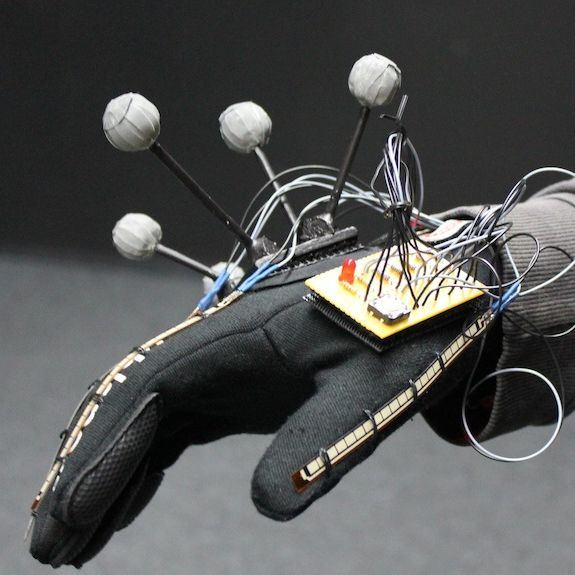
\includegraphics[width=\textwidth]{figs/glove}
      \tiny{\textbf{\\Fonte: \citeonline{luva_mocap}}}
    \end{column}

    \begin{column}{.3\textwidth}
      \centering
      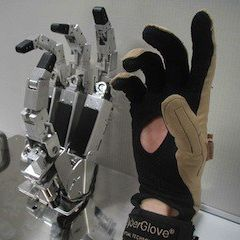
\includegraphics[width=\textwidth]{figs/cyberglove}
      \tiny{\textbf{\\Fonte: \citeonline{cyberglove}}}
    \end{column}

    \begin{column}{.3\textwidth}
      \centering
      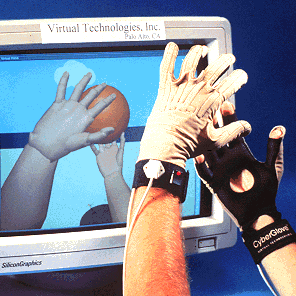
\includegraphics[width=\textwidth]{figs/cyberglove2}
      \tiny{\textbf{\\Fonte: \citeonline{cyberglove2}}}
    \end{column}
  \end{columns}
}

\frame{
  \frametitle{Problemas tratados}
  \begin{columns}
    \begin{column}{.6\textwidth}
      \begin{itemize}
        \item Custo;
          \note[item]{Luvas existentes são caras, podendo custar de US\$250,00 até US\$12.995,00.}
          \note[item]{Redução de custos com componentes acessíveis.}
        \item Complexidade dos movimentos;
          \note[item]{Possibilitar realização de movimentos mais complexos permite uso em mais cenários diferentes, como tradução de linguagem de sinais ou VR}
        \item Melhoria do protótipo de \citeonline{roversi}.
          \note[item]{este trabalho é uma continuação do trabalho de Roversi.}
          \note[item]{O protótipo original só capta flexão e extensão dos dedos e do pulso.}
          \note[item]{Incluir mais movimentos.}
      \end{itemize}
      \centering
      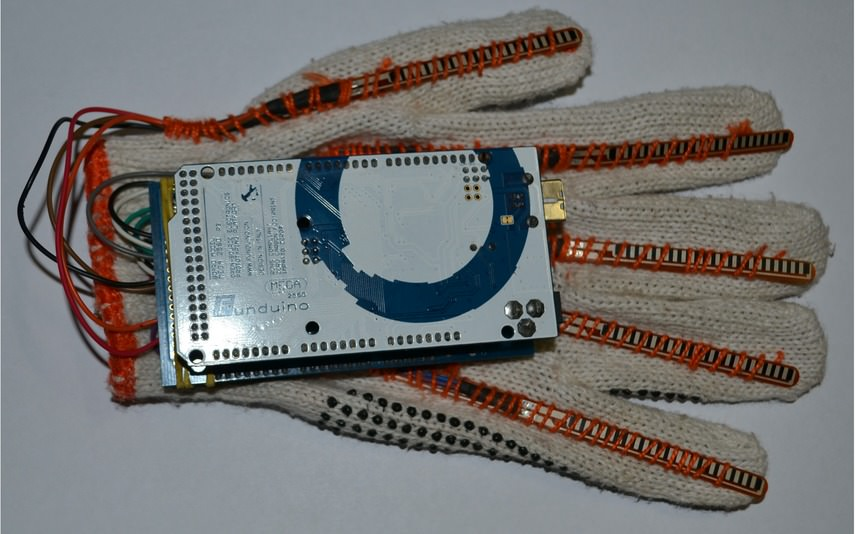
\includegraphics[width=.7\textwidth]{figs/2016roversi}
      \tiny{\textbf{\\Fonte: \citeonline{roversi}}}
    \end{column}

    \begin{column}{.4\textwidth}
      \centering
      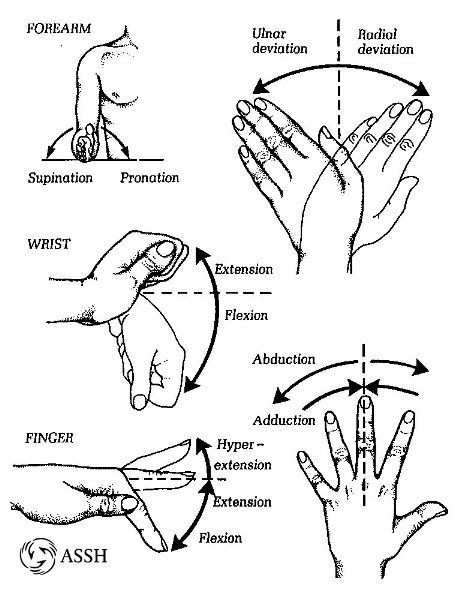
\includegraphics[width=\textwidth]{figs/movimentos}
      \tiny{\textbf{\\Fonte: \citeonline{movimentos}}}
    \end{column}
  \end{columns}
}


\frame{
  \frametitle{Objetivos e Justificativas}
  \begin{itemize}   
     \item Objetivos
     \begin{itemize}
        \item Movimentos de adução e abdução dos dedos;
          \note[item]{Abdução - Abrir; Adução - Fechar}
        \item Movimentos de desvios radial e ulnar do pulso;
          \note[item]{Desvio Radial - Na direção do polegar; Ulnar - Na direção do dedo mínimo}
        \item Redução de ruídos dos sensores.
          \note[item]{O protótipo de Roversi possuía muitos ruídos}
     \end{itemize}
     
     \item Justificativas
     \begin{itemize}
        \item Controle de braços robóticos;
        \item Captura de movimentos para animações;
        \item Reconhecimento de gestos;
          \note[item]{Linguagem de sinais}
        \item Realidade virtual.
     \end{itemize}
 \end{itemize}
}


\section{Revisão de Literatura}
\frame{
  \frametitle{Sensores}
  \note[item]{Pesquisa dos sensores mais utilizados em luvas eletrônicas}
  \note[item]{Serão detalhados nos próximos slides}
  \begin{columns}
    \begin{column}{.6\textwidth}
      \begin{itemize}%
      \item Sensor de Flexão
      \item IMU (Unidade de Medição Inercial)%
      \begin{itemize}%
        \item Acelerômetro
        \item Giroscópio
        \item Magnetômetro
      \end{itemize}
    \end{itemize}
    \end{column}
    \begin{column}{.4\textwidth}
      \centering
      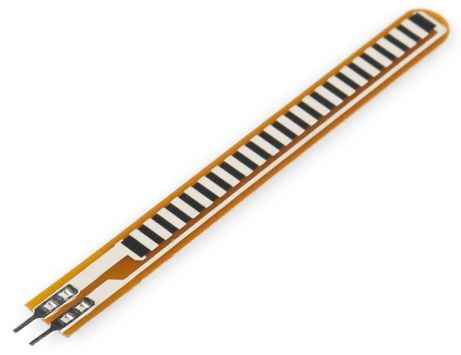
\includegraphics[height=.3\textheight]{figs/spectraFlex}
      \tiny{\textbf{\\Fonte: \citeonline{sparkflex}}}
      \\\quad
      \\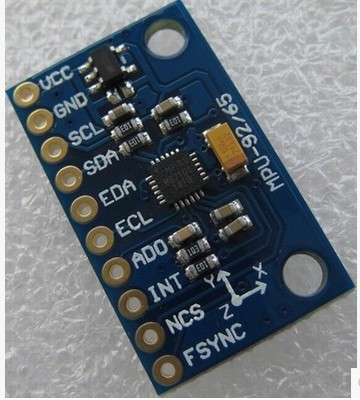
\includegraphics[height=.3\textheight]{figs/mpu9250}
      \tiny{\textbf{\\Fonte: \citeonline{mpu9250}}}
    \end{column}
  \end{columns}
}

\frame{
  \frametitle{Sensor de Flexão}
  \note[item]{Quando dobrado aumenta resistência}
  \note[item]{Partículas condutivas se afastam, dificultando a passagem de corrente}
  \begin{columns}
    \begin{column}{.5\textwidth}
    \begin{itemize}
      \item Detecta dobras
      \item Baseado em tinta resistiva
    \end{itemize}
      \centering
      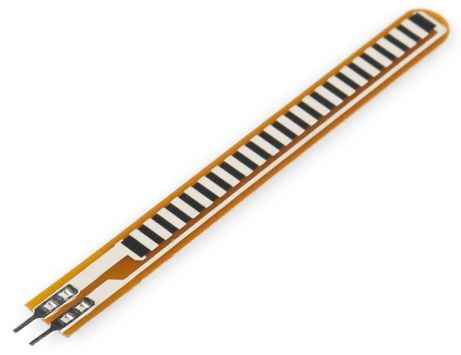
\includegraphics[width=.7\textwidth]{figs/spectraFlex}
      \tiny{\textbf{\\Fonte: \citeonline{sparkflex}}}
    \end{column}
    \begin{column}{.5\textwidth}
      \centering
      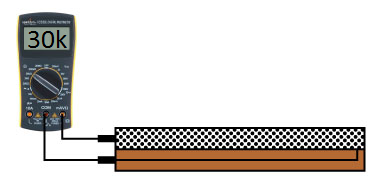
\includegraphics[height=.3\textheight]{figs/sensor_reto.png}
      \\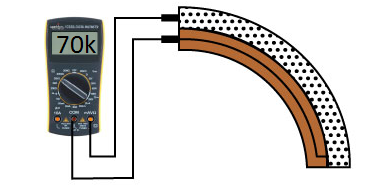
\includegraphics[height=.3\textheight]{figs/sensor_curvo.png}
      \tiny{\textbf{\\Fonte: \citeonline{sparkflex}}}
    \end{column}
  \end{columns}
}

\frame{
  \frametitle{Acelerômetro}
  \note[item]{Possui uma massa móvel, suspensa por molas, que se desloca com o movimento gerando um sinal elétrico}
  \note[item]{Em descanso sobre uma superfície plana, mede aceleração de 9.8 m/s2 sobre o eixo vertical}
  \note[item]{Em queda livre, mede 0 m/s2}
  \begin{columns}
    \begin{column}{.5\textwidth}
      \begin{itemize}
        \item Detecta aceleração exercida sobre o dispositivo;
        \item Ideal para detecção de movimentos de translação;
        \item Leituras ruidosas. 
      \end{itemize}
    \end{column}
    \begin{column}{.5\textwidth}
      \centering
      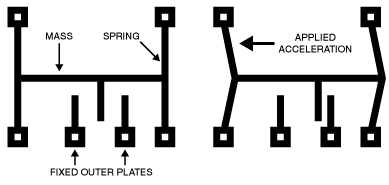
\includegraphics[height=.3\textheight]{figs/accel}
      \tiny{\textbf{\\Fonte: \citeonline{accel}}}
    \end{column}
  \end{columns}
}

\frame{
  \frametitle{Giroscópio}
  \note[item]{Velocidade angular é a taxa de variação do ângulo de rotação em torno de um eixo.}
  \note[item]{Possui uma massa que oscila verticalmente}
  \note[item]{quando rotacionado, a força de Coriolis age sobre a massa, fazendo-a movimentar horizontalmente}
  \note[item]{A força de Coriolis é uma força que surge num sistema referencial em rotação e que tende a alterar a trajetória dos corpos em movimento.}
  \begin{columns}
    \begin{column}{.5\textwidth}
      \begin{itemize}
        \item Detecta velocidade angular;
        \item Ideal para detecção de movimentos de rotação;
        \item Leituras pouco ruidosas;
        \item Suscetível a acúmulo de erros ao longo do tempo (\textit{drift}). 
      \end{itemize}
    \end{column}
    \begin{column}{.5\textwidth}
      \centering
      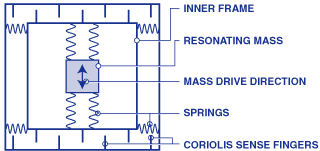
\includegraphics[height=.3\textheight]{figs/gyro_vsg1}
      \tiny{\textbf{\\Fonte: \citeonline{gyroscope}}}
    \end{column}
  \end{columns}
}

\frame{
  \frametitle{Magnetômetro}
  \note[item]{ o efeito de Hall se refere ao desvio da trajetória normal das cargas fluindo em um semicondutor, quando este é submetido à ação de um campo magnético. Este desvio causa uma diferença de potencial que pode ser medida perpendicularmente ao sentido do movimento da corrente}
  \begin{columns}
    \begin{column}{.5\textwidth}
      \begin{itemize}
        \item Detecta o campo magnético ao redor do dispositivo;
        \item Utiliza o efeito de Hall como princípio de funcionamento;
        \item Sofre influência de campos magnéticos externos.
      \end{itemize}
    \end{column}
    \begin{column}{.5\textwidth}
      \centering
      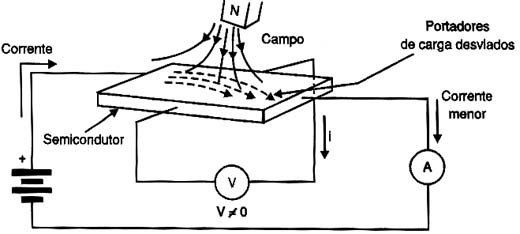
\includegraphics[height=.3\textheight]{figs/hall}
      \tiny{\textbf{\\Fonte: \citeonline{hall}}}
    \end{column}
  \end{columns}
}

\frame{
  \frametitle{Trabalhos Relacionados}
  \note[item]{Serão apresentados alguns trabalhos relacionados com o tema de captura de movimentos da mão.}
  \begin{columns}
    \begin{column}{.3\textwidth}
      \begin{itemize}
        \item \textit{KHU-1}
      \end{itemize}
      \centering
      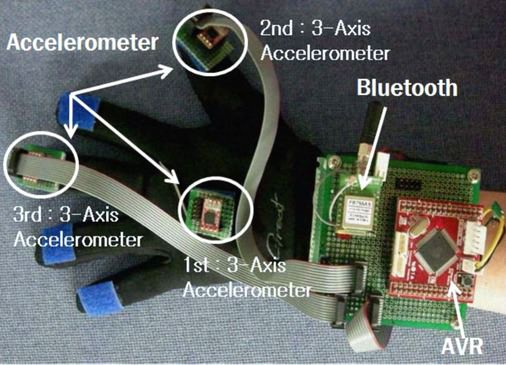
\includegraphics[width=\textwidth]{figs/2009accel}
      \tiny{\textbf{\\Fonte: \citeonline{kim20093}}}
    \end{column}
    \begin{column}{.3\textwidth}
      \begin{itemize}
        \item \textit{Smartglove}
      \end{itemize}
      \centering
      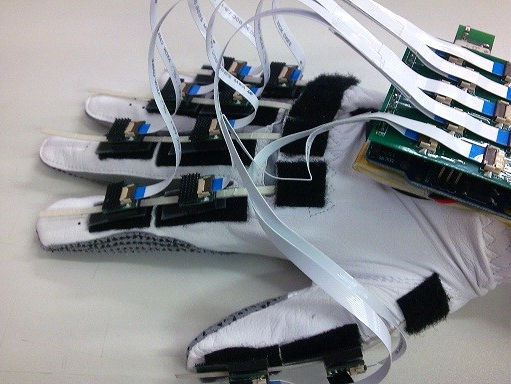
\includegraphics[width=\textwidth]{figs/smartglove2}
      \tiny{\textbf{\\Fonte: \citeonline{li2009smartglove}}}
    \end{column}
    \begin{column}{.3\textwidth}
      \begin{itemize}
        \item \citeonline{roversi}
      \end{itemize}
      \centering
      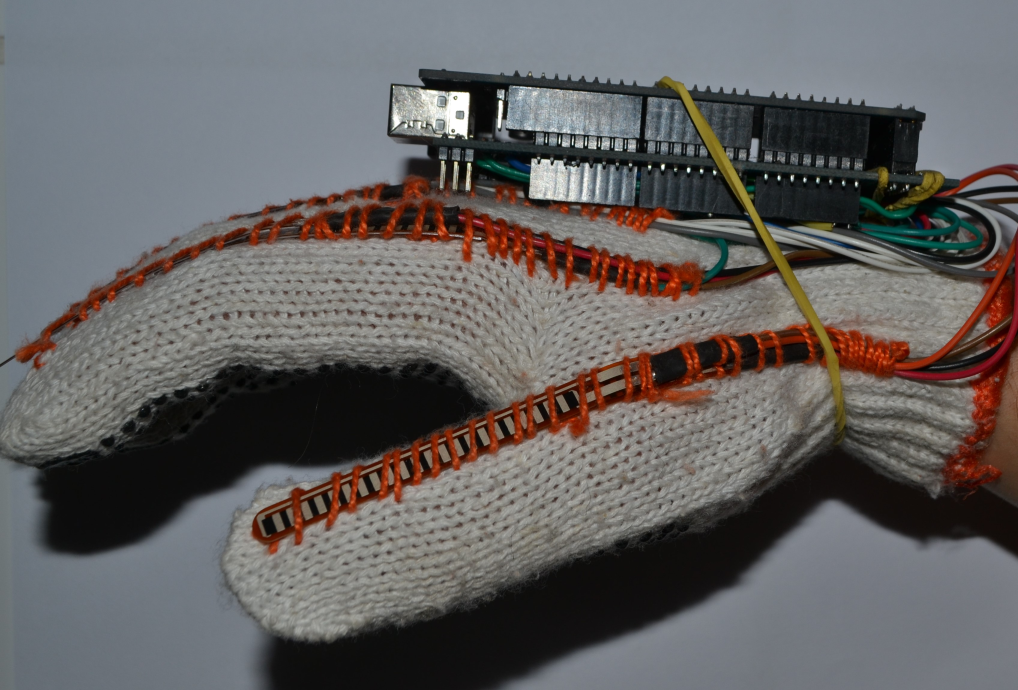
\includegraphics[width=\textwidth]{figs/roversi}
      \tiny{\textbf{\\Fonte: \citeonline{roversi}}}
    \end{column}
  \end{columns}
}

\frame{
  \frametitle{\textit{KHU-1}}
  \begin{itemize}
    \item 3 \textit{IMUs}
    \item Reconhecimento dos gestos de "pedra", "papel" e "tesoura"
    \item Não reconhece movimentos dos dedos individualmente
  \end{itemize}
  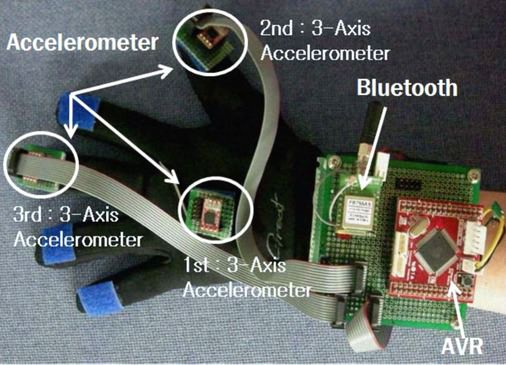
\includegraphics[height=.4\textheight]{figs/2009accel}
  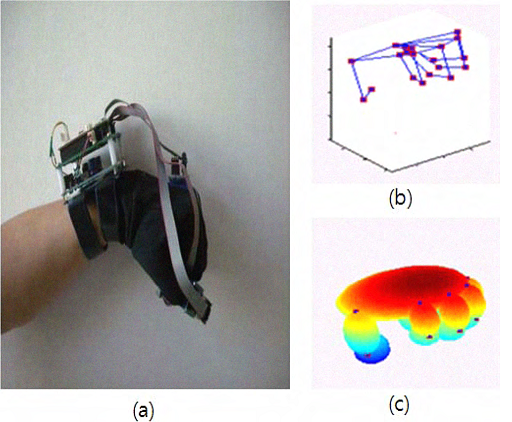
\includegraphics[height=.4\textheight]{figs/khu1}
  \centering
  \tiny{\textbf{\\Fonte: \citeonline{kim20093}}}
}

\frame{
  \frametitle{\textit{Smartglove}}
  \begin{itemize}
    \item 10 transdutores lineares ópticos
    \item Boa repetibilidade dos movimentos
    \item Não detecta movimentos do pulso ou de abdução dos dedos
  \end{itemize}
  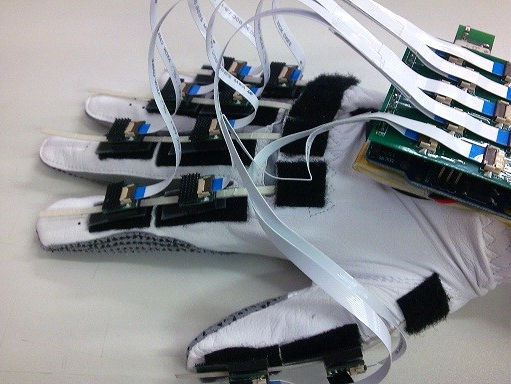
\includegraphics[height=.4\textheight]{figs/smartglove2}
  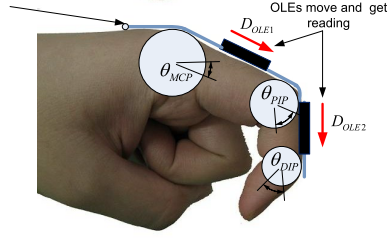
\includegraphics[height=.4\textheight]{figs/2009smartglove}
  \centering
  \tiny{\textbf{\\Fonte: \citeonline{li2009smartglove}}}

}

\frame{
  \frametitle{\textit{\citeonline{roversi}}}
  \begin{itemize}
    \item 10 sensores de flexão
    \item 1 IMU
    \item Detecta flexão e extensão dos dedos e do pulso
    \item Muitos ruídos
  \end{itemize}
  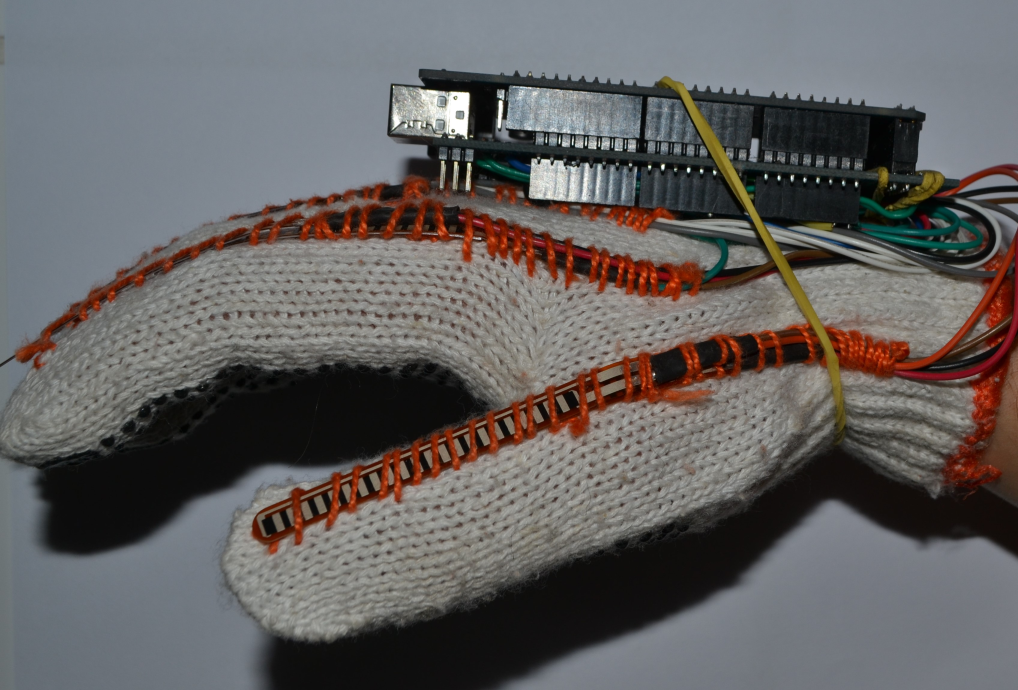
\includegraphics[height=.4\textheight]{figs/roversi}
  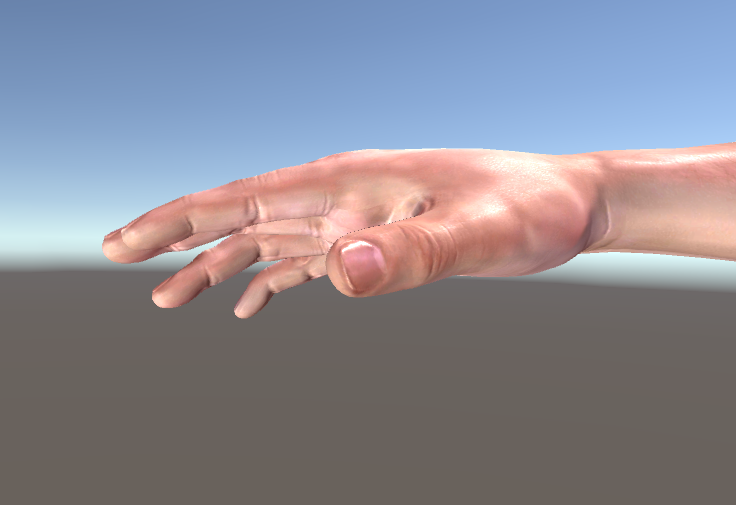
\includegraphics[height=.4\textheight]{figs/roversi2}
  \centering
  \tiny{\textbf{\\Fonte: \citeonline{roversi}}}

}

\section{Metodologia}
\frame{
  \frametitle{\textit{Hardware}}
  \begin{columns}
    \begin{column}{.4\textwidth}
      \begin{itemize}
        \item \textit{Arduino Mega}
          \note[item]{Arduino Mega foi escolhido devido ao número de portas analógicas (16)}
        \item 14 Sensores de flexão
          \note[item]{Sensor de flexão foi escolhido pela facilidade de uso e disponibilidade}
        \item 2 \textit{MPU-9250}
          \note[item]{MPU-9250 foi escolhida por ter acelerômetro giroscópio e magnetômetro, sendo possível a fusão dos sensores}
          \note[item]{MPU-6050 possui apensa acelerômetro e giroscópio}
      \end{itemize}
    \end{column}
    \begin{column}{.6\textwidth}
      \centering
      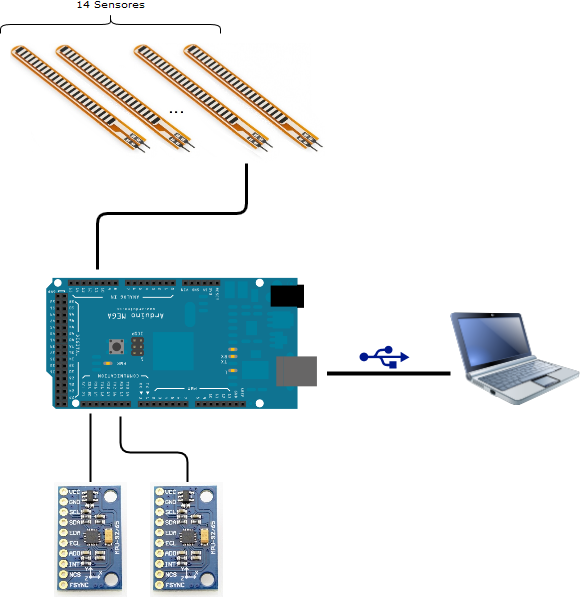
\includegraphics[width=\textwidth]{figs/arquitetura}
      \tiny{\textbf{\\Fonte: Autor}}
    \end{column}
  \end{columns}
}

\frame{
  \frametitle{Circuito}
  \note[item]{Sensores de flexão nos pinos analógicos}
  \note[item]{Resistores de 10K fazendo divisor de tensão}
  \note[item]{Conexão das IMUs nos pinos SCL e SDA do protocolo I2C}
  \note[item]{Pino AD0 das IMUs conectado em 3.3V ou GND, para definição do endereço I2C}
  \centering
  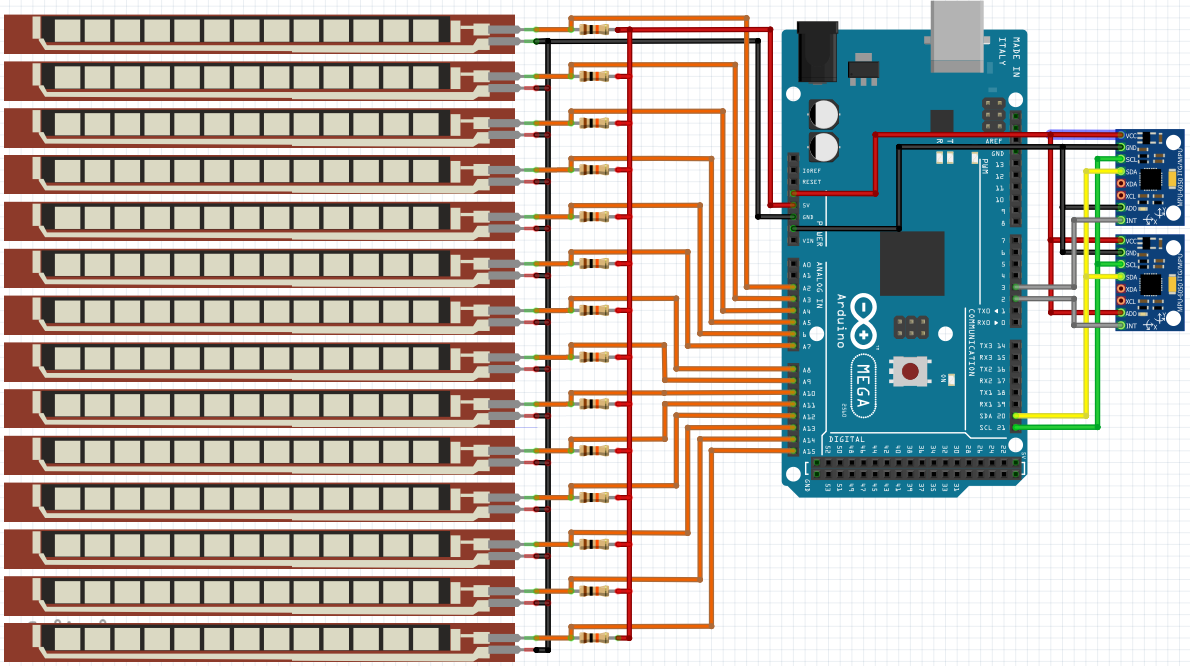
\includegraphics[width=\textwidth]{figs/fritzingtudo.png}
  \tiny{\textbf{\\Fonte: Autor}}
}

\frame{
  \frametitle{Circuito}
  \note[item]{Sensores de flexão nos pinos analógicos}
  \note[item]{Resistores de 10K fazendo divisor de tensão}
  \note[item]{Conexão das IMUs nos pinos SCL e SDA do protocolo I2C}
  \note[item]{Pino AD0 das IMUs conectado em 3.3V ou GND, para definição do endereço I2C}
  \centering
  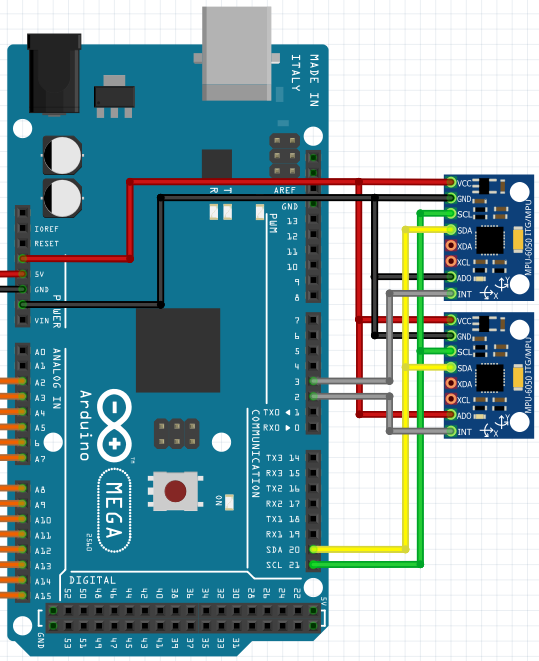
\includegraphics[width=.8\textheight,angle=90]{figs/fritzingmpu.png}
  \tiny{\textbf{\\Fonte: Autor}}
}

\frame{
  \frametitle{\textit{Software}}
  \begin{itemize}
    \item \textit{Unity 3D}
      \note[item]{Unity foi usada para modelagem e visualização dos movimentos e recepção dos dados}
    \item \textit{Arduino IDE}
      \note[item]{Arduino IDE foi usada para implementação dos códigos do Arduino}
  \end{itemize}
  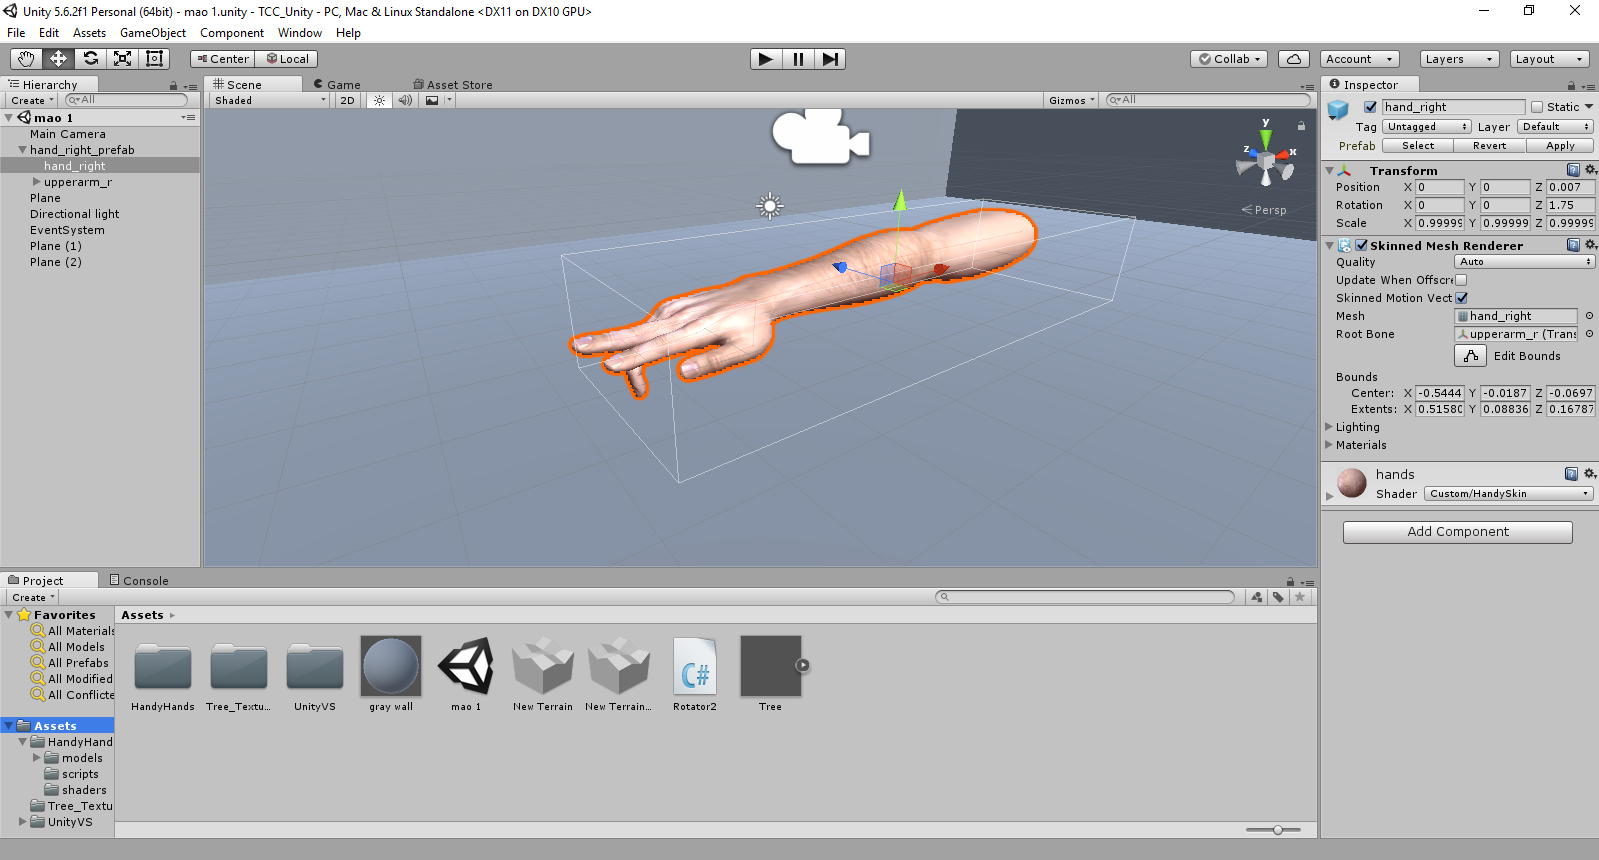
\includegraphics[height=.45\textheight]{figs/tut_unity}
  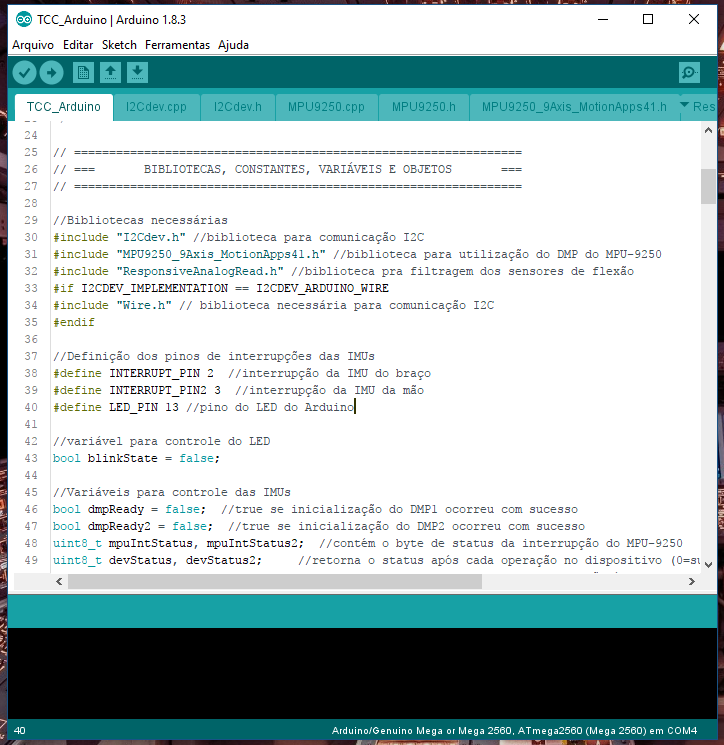
\includegraphics[height=.45\textheight]{figs/tut_ard}
  \centering
  \tiny{\textbf{\\Fonte: Autor}}
}

\frame{
  \frametitle{Disposição dos sensores}
  \note[item]{Sensores de flexão posicionados sobre as articulações}
  \note[item]{sensores de abdução posicionados entre os dedos}
  \note[item]{detecção das articulações IFD e IFP com um sensor}
  \note[item]{posicionamento das IMUs para captar movimentos do pulso}
  \begin{columns}
    \begin{column}{.4\textwidth}
      \centering
      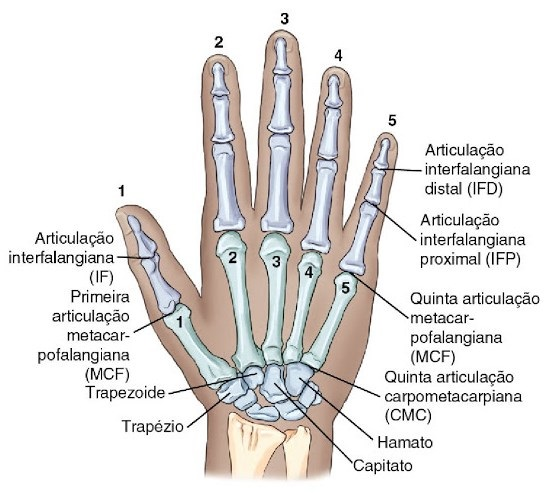
\includegraphics[width=\textwidth]{figs/articulacoes}
      \tiny{\textbf{\\Fonte: \citeonline{articulacoes}}}
    \end{column}
    \begin{column}{.7\textwidth}
      \centering
      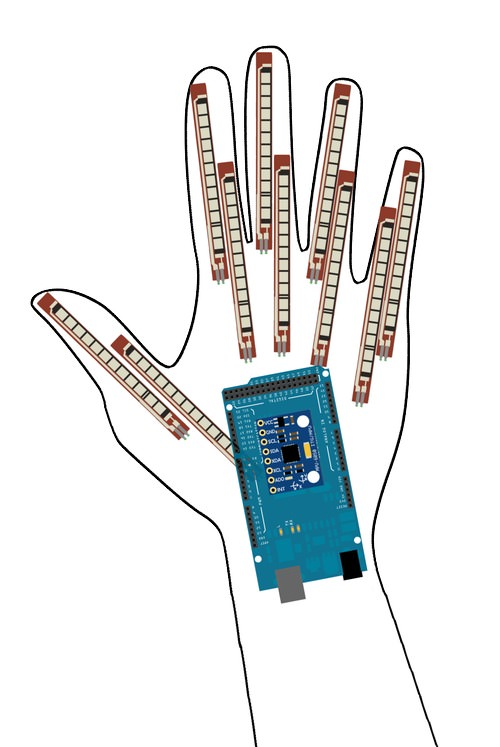
\includegraphics[height=.6\textheight]{figs/Luva_Atual}
      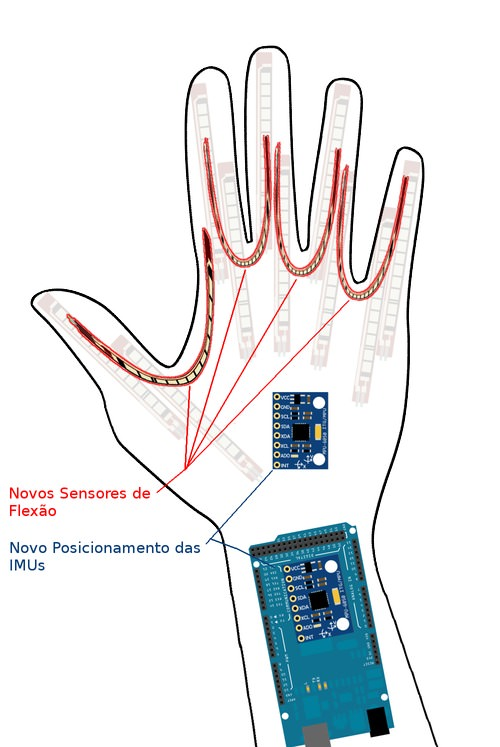
\includegraphics[height=.6\textheight]{figs/Nova_Luva}
      \tiny{\textbf{\\Fonte: Autor}}
    \end{column}
  \end{columns}
}

\frame{
  \frametitle{Casos de Teste}
  \note[item]{Desvio Padrão e Amplitude para analisar os resultados dos filtros}
  \note[item]{Xs - conjunto de amostras do sensor S, n - número de amostras}
  \note[item]{DMA para analisar a precisão dos movimentos}
  \note[item]{Vr - valor real, Vc - valor calculado}
  \note[item]{DMA calculado com os ângulos real e após conversão pelo Arduino}
  \begin{columns}
    \begin{column}{.5\textwidth}
      \begin{itemize}
        \item Desvio Padrão:
        \begin{equation*}
          \delta_S = \sqrt{\frac{\sum_{i=1}^n(X_{S_i} - \overline{X_S})^2}{n-1}}
        \end{equation*}
        \item Amplitude:
        \begin{equation*}
          R_S = \max(X_{S_i}) - \min(X_{S_i})
        \end{equation*}
        \item Desvio Médio Absoluto:
        \begin{equation*}
          DMA = \frac{\sum_{i=1}^n\lvert V_r - V_c \rvert}{n}
        \end{equation*}
      \end{itemize}
    \end{column}
    \begin{column}{.5\textwidth}
      \centering
      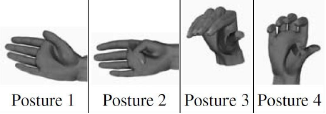
\includegraphics[width=\textwidth]{figs/posicoes}\\
      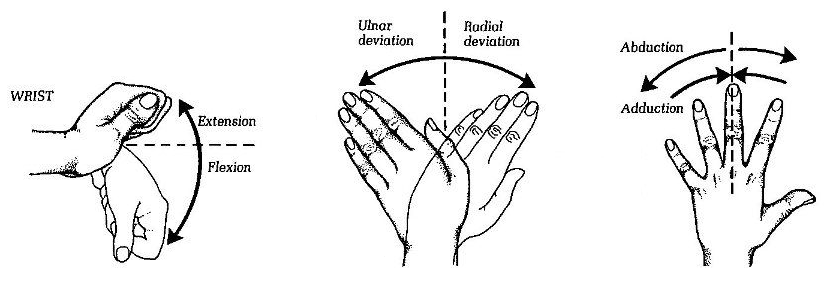
\includegraphics[width=\textwidth]{figs/posicoes2}
      \tiny{\textbf{\\Fonte: \citeonline{li2009smartglove}, \citeonline{movimentos}}}
    \end{column}
  \end{columns}
}

\section{Desenvolvimento}
\frame{
  \frametitle{Luva}
  \note[item]{Utilizada em esportes aquáticos e é bem resistente}
  \begin{columns}
    \begin{column}{.5\textwidth}
      \begin{itemize}
        \item Luva de neoprene
        \item Permite boa fixação dos sensores
        \item Tecido não desloca durante os movimentos
      \end{itemize}
    \end{column}
    \begin{column}{.5\textwidth}
      \centering
      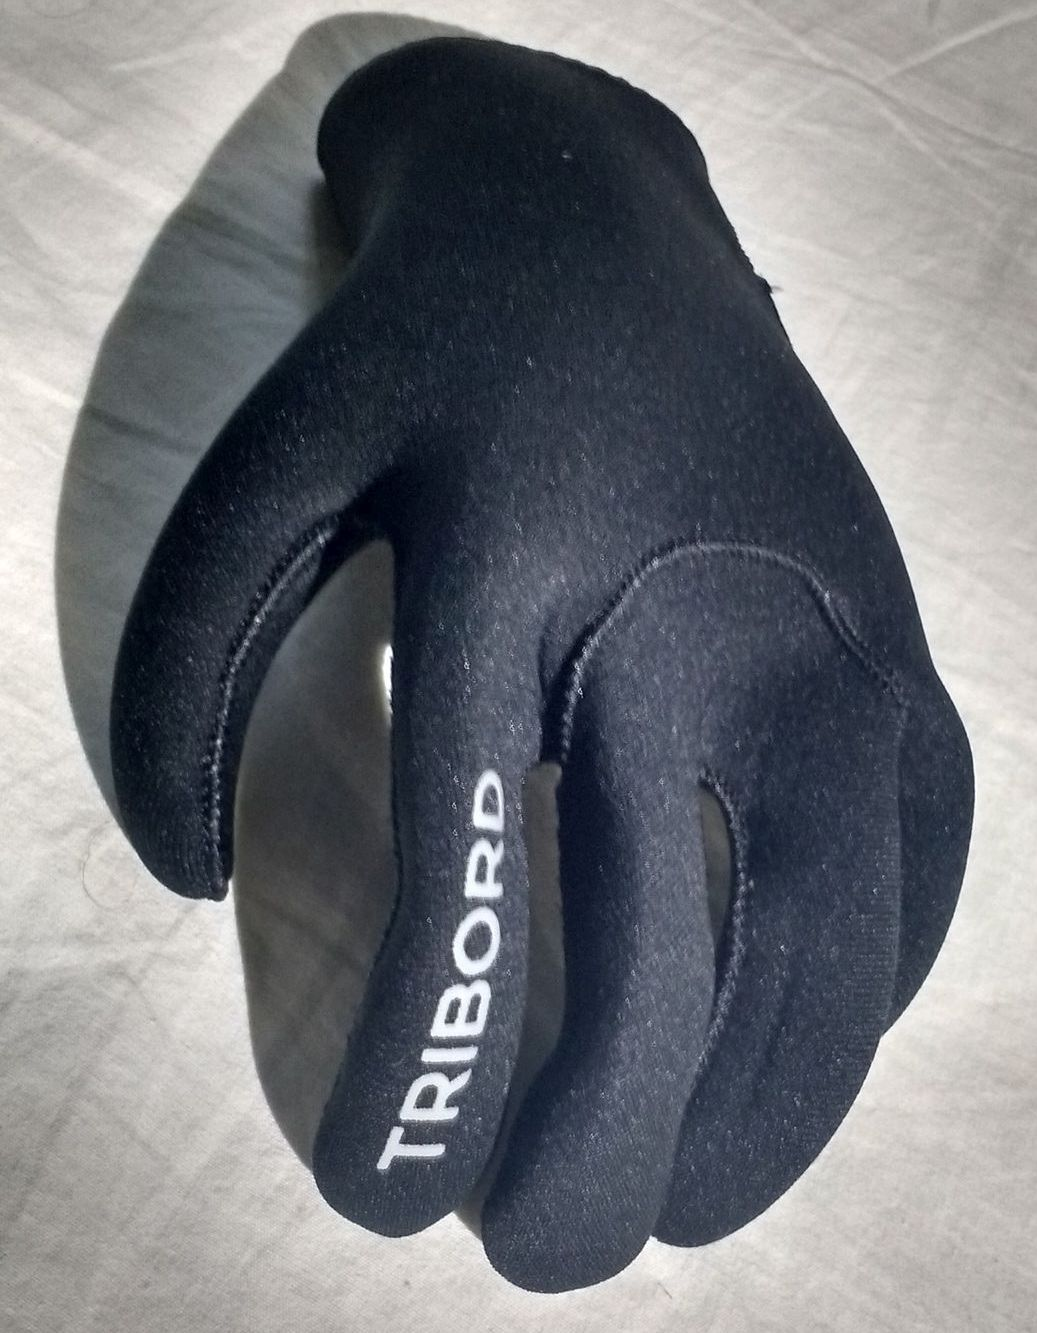
\includegraphics[width=.7\textwidth]{figs/luvaneoprene.jpg}
      \tiny{\textbf{\\Fonte: Autor}}
    \end{column}
  \end{columns}
}

\frame{
  \frametitle{Sensores de flexão}
  \begin{columns}
  \begin{column}{.6\textwidth}
    \begin{itemize}
      \item Fixados com costura
      \item Posicionados sobre as articulações do dedos
      \item Sensores de adução e abdução entre os dedos
      \item Ângulo de dobra dado pela variação da resistência
    \end{itemize}
  \end{column}
  \begin{column}{.4\textwidth}
    \centering
      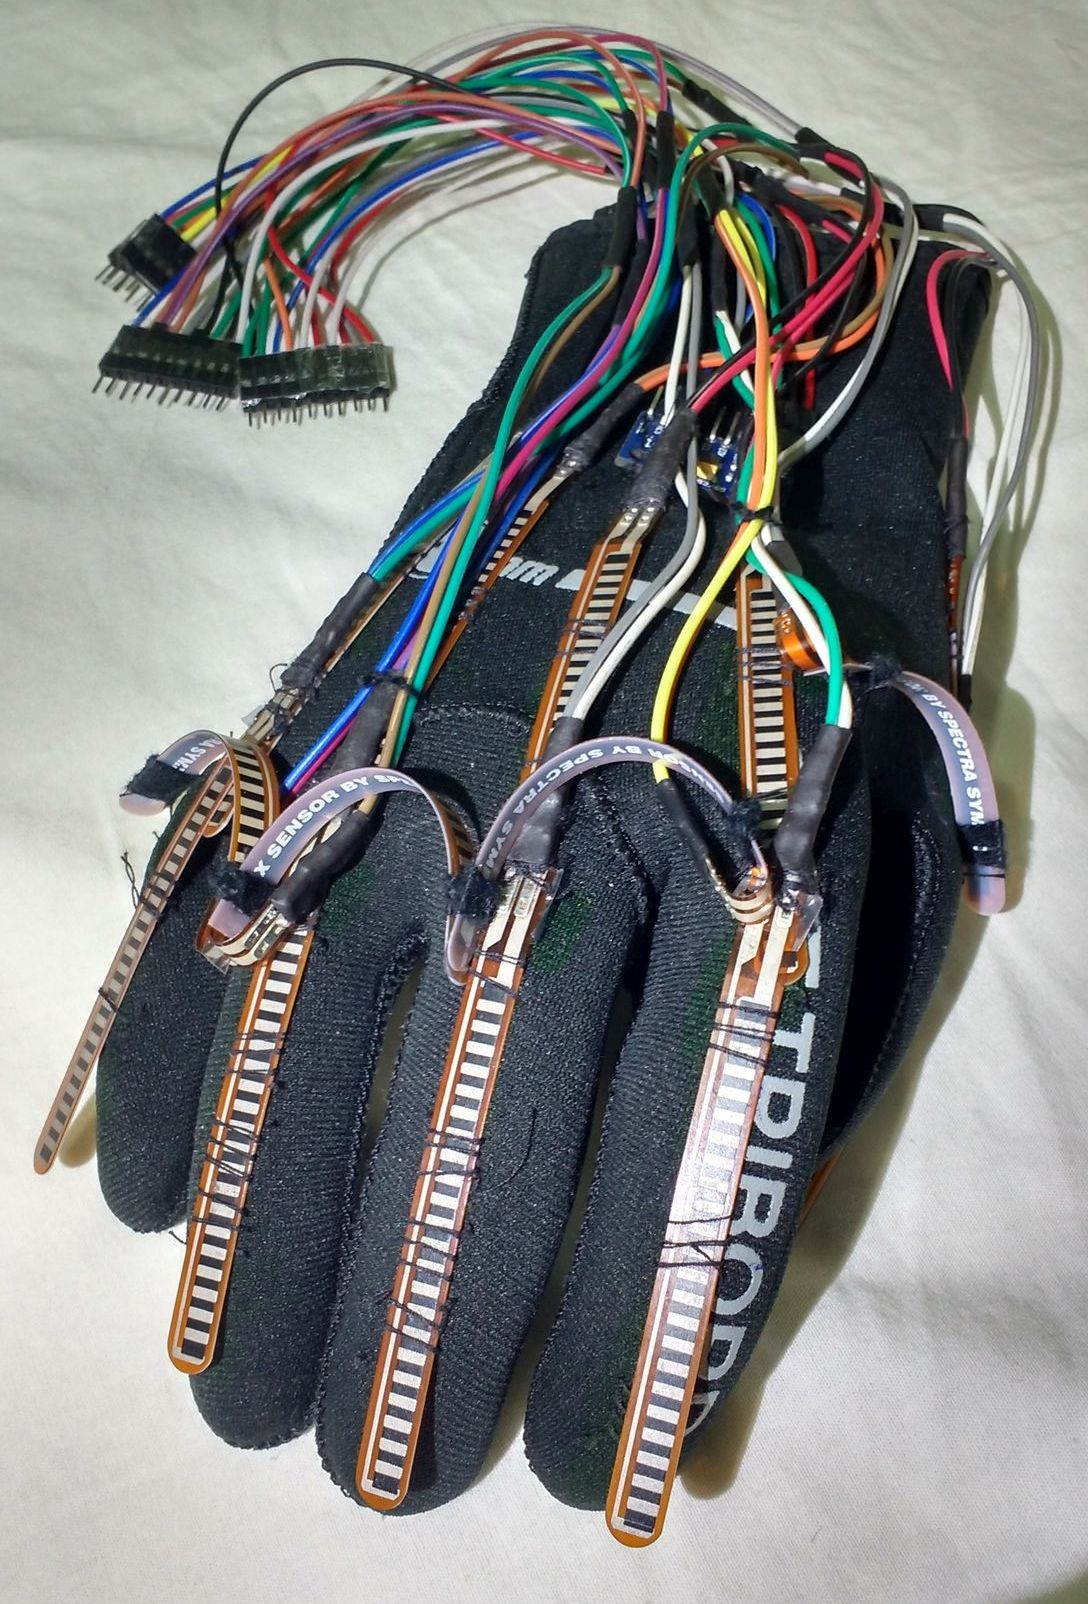
\includegraphics[width=\textwidth]{figs/LuvaFrente}
      \tiny{\textbf{\\Fonte: Autor}}
  \end{column}
  \end{columns}
}

\frame{
  \frametitle{\textit{IMUs}}
    \begin{columns}
    \begin{column}{.6\textwidth}
      \begin{itemize}
        \item Posicionados nas costas da mão e no antebraço
        \item Fixado com costura na luva
        \item Ângulo de dobra do pulso dado pela diferença da orientação entre as duas \textit{IMUs}
      \end{itemize}
    \end{column}
    \begin{column}{.4\textwidth}
      \centering
        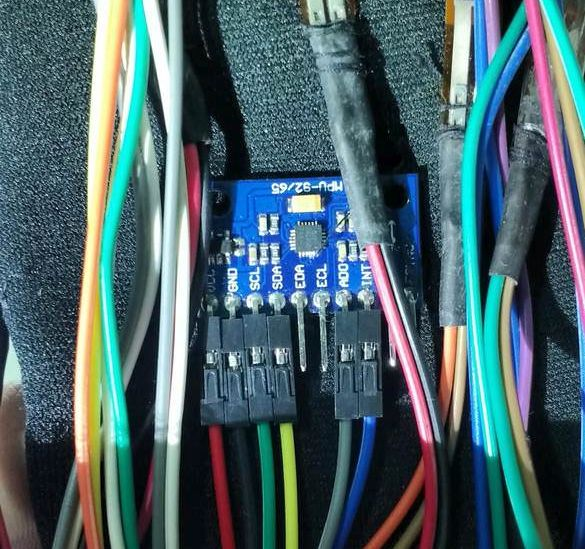
\includegraphics[width=\textwidth]{figs/detalheIMU}
        \tiny{\textbf{\\Fonte: Autor}}
    \end{column}
    \end{columns}
}

\frame{
  \frametitle{Circuito}
  \note[item]{Conectores facilitam retirada dos sensores}
  \note[item]{Testes foram realizados com o circuito de Roversi e com o novo circuito}
  \begin{itemize}
      \item Shield de prototipagem
    \item Conectores de barra para facilitar testes
  \end{itemize}
  \centering
    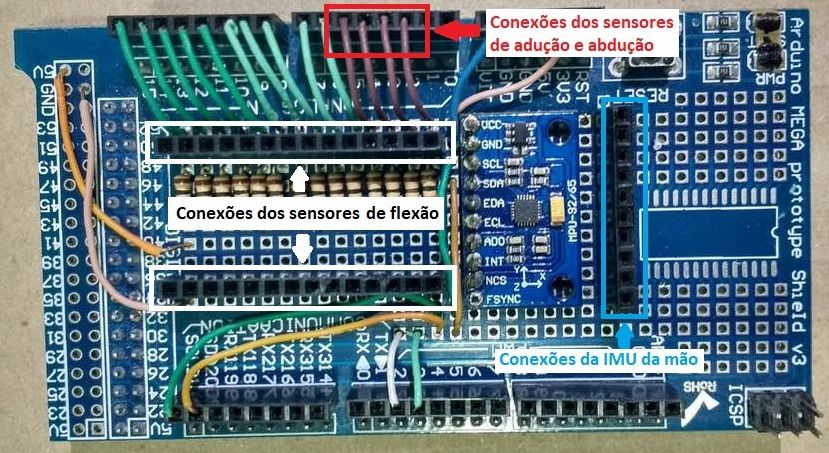
\includegraphics[height=.5\textheight]{figs/placaCima}
    \tiny{\textbf{\\Fonte: Autor}}
}

\frame{
  \frametitle{Luva finalizada}
  \note[item]{Fixação do Arduino no braço não foi ideal}
  \begin{itemize}
      \item Luva de \textit{lycra} auxilia na fixação e dobra dos sensores
  \end{itemize}
    \centering
    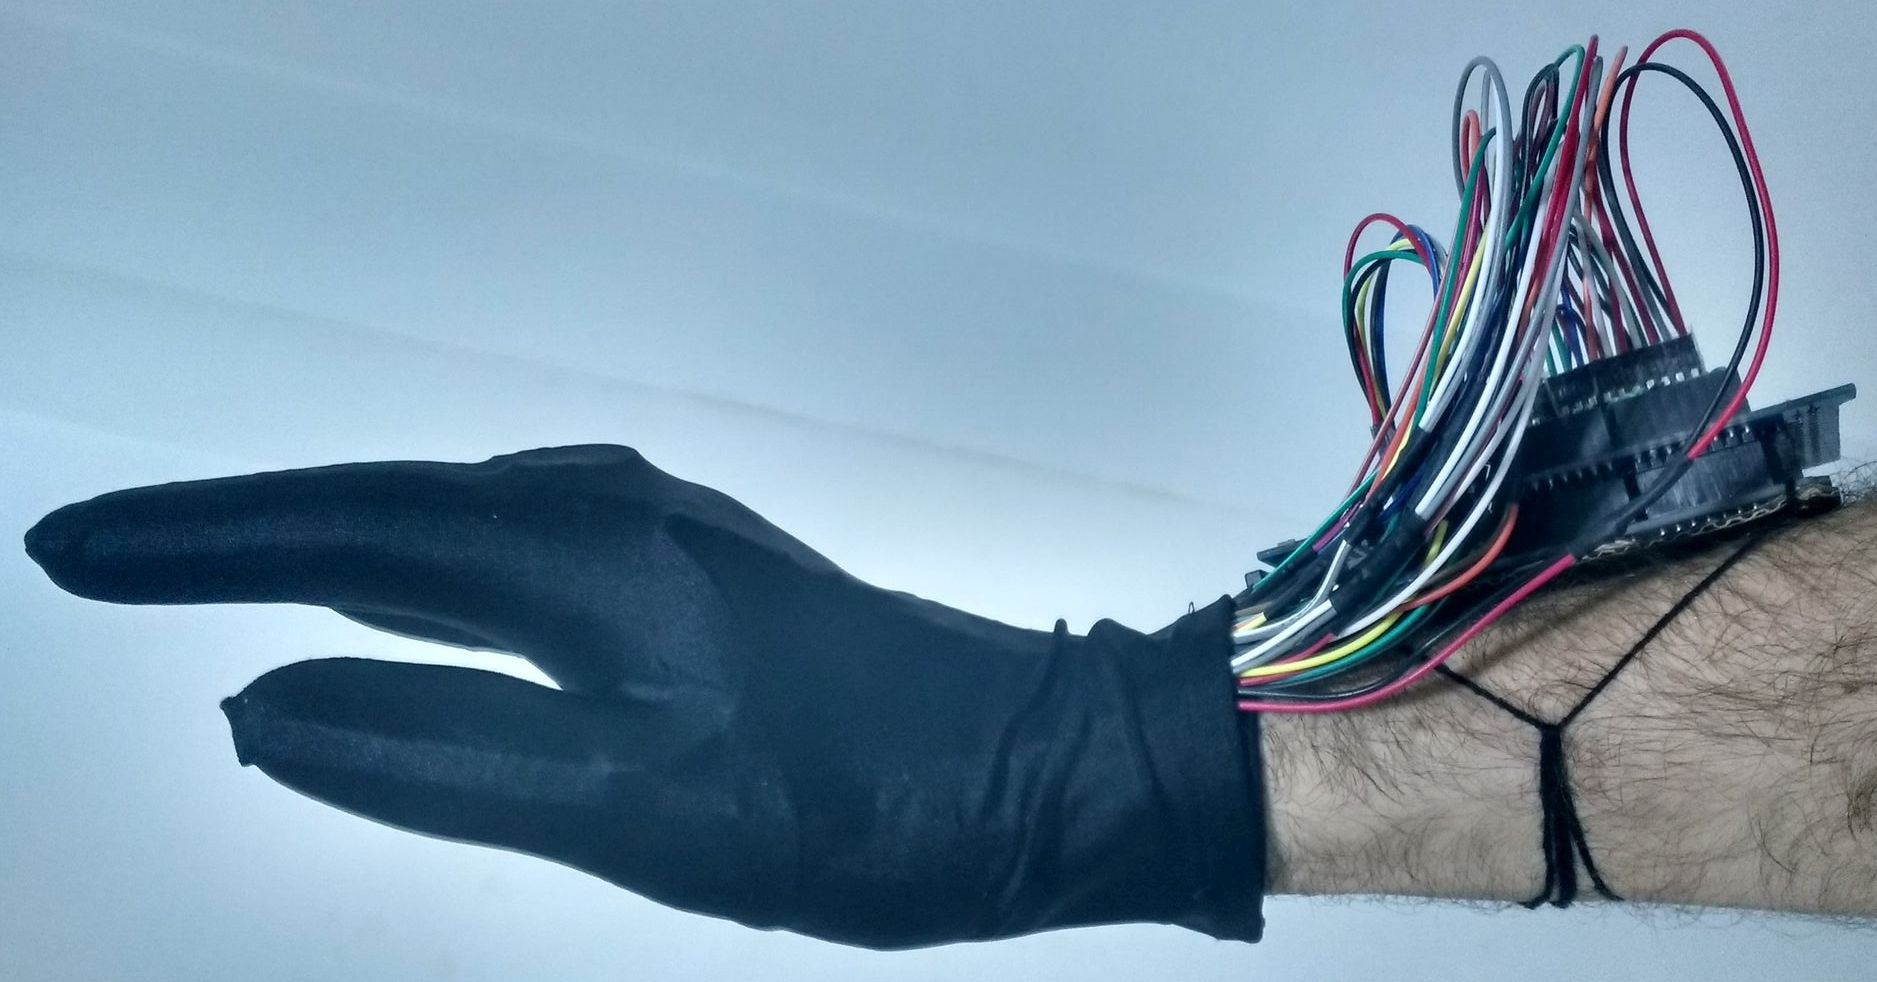
\includegraphics[width=.7\textwidth]{figs/luvanamaolateral.jpg}
    \tiny{\textbf{\\Fonte: Autor}}
}

\frame{
  \frametitle{Códigos}
\note[item]{Biblioteca ResponsiveAnalogRead usada para filtro dos sensores de flexão}
\note[item]{Filtro média móvel exponencial que dá mais peso às leituras mais recentes}
\note[item]{IMU protocolo I2C}
\note[item]{DMP usado para fusão das leituras do acelerômetro, giroscópio e magnetômetro}
\note[item]{Comunicação unity via porta serial USB}
  \begin{itemize}
  \item \textit{Arduino}
  \begin{itemize}
      \item Aquisição dos dados
      \item Conversões para ângulos
      \item Envio pela porta serial
    \end{itemize}
  \item \textit{Unity}
    \begin{itemize}
      \item Recebimento dos dados
      \item Movimentação dos elementos
    \end{itemize}
    \end{itemize}
}

\frame{
  \frametitle{Diagrama de Sequência}
  \note[item]{Unity requisita dados do Arduino a cada atualização de frame}
  \note[item]{Aquisição dos dados de orientação das IMUs no formato de quatérnios, devido a leituras errôneas com formato de ângulos de Euler}
  \note[item]{Quatérnios são representações de orientação no espaço utilizando 4 coordenadas complexas}
  \centering
  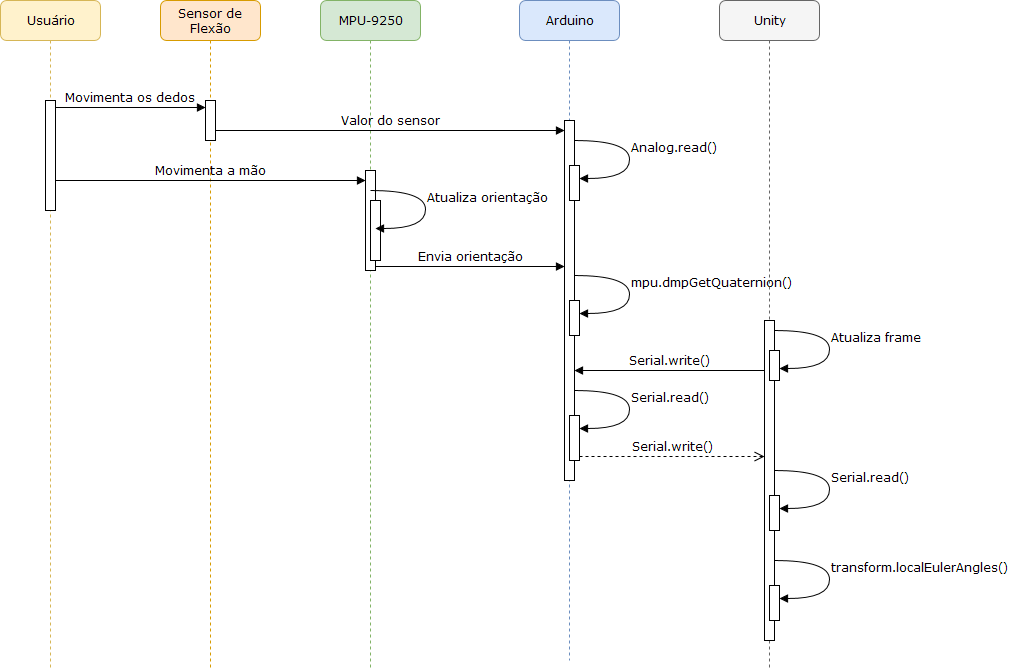
\includegraphics[width=\textwidth]{figs/sequencia.png}
  \tiny{\textbf{\\Fonte: Autor}}
}

\frame{
  \frametitle{Fluxograma}
  \centering
  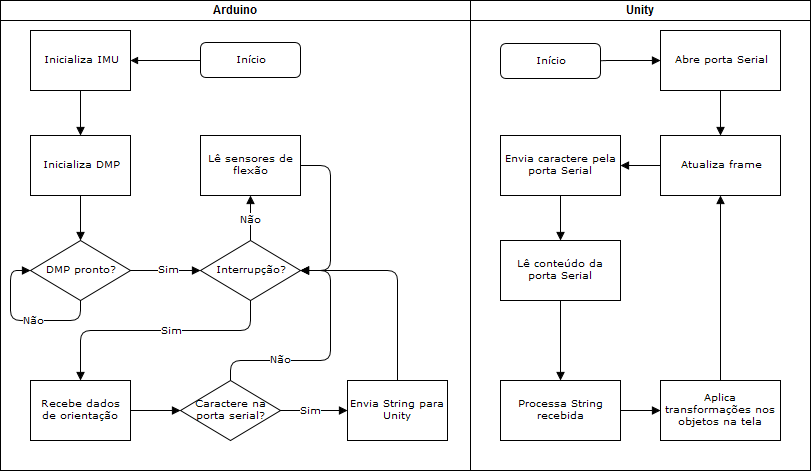
\includegraphics[width=\textwidth]{figs/processos.png}
  \tiny{\textbf{\\Fonte: Autor}}
}

\section{Resultados}
\frame{
  \frametitle{Filtro dos sensores de flexão}
  \note[item]{Leituras das articulações MCF e IF do polegar na posição plana}
  \begin{columns}
    \begin{column}{\paperwidth}
      \centering
      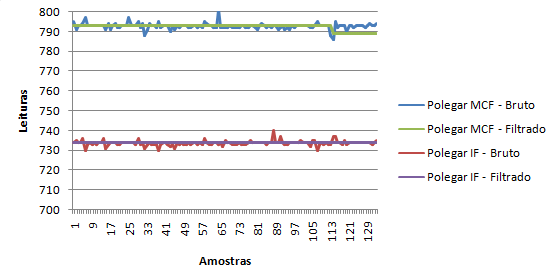
\includegraphics[height=.7\textheight]{figs/sensflex_pol1-2_filtrado_bruto_meu.png}
      \tiny{\textbf{\\Fonte: Autor}}
    \end{column}
    \end{columns}
}

\frame{
  \frametitle{Leituras das \textit{IMUs}}
  \note[item]{Leituras das IMus sobre superfície plana}
  \begin{columns}
    \begin{column}{\paperwidth}
      \centering
      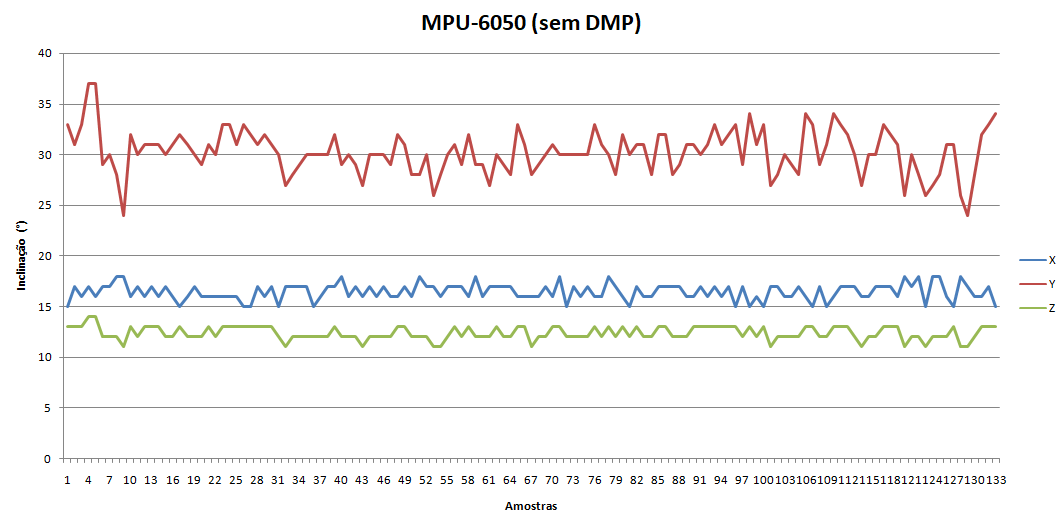
\includegraphics[height=.4\textheight]{figs/6050nodmp_plano.png}\\
      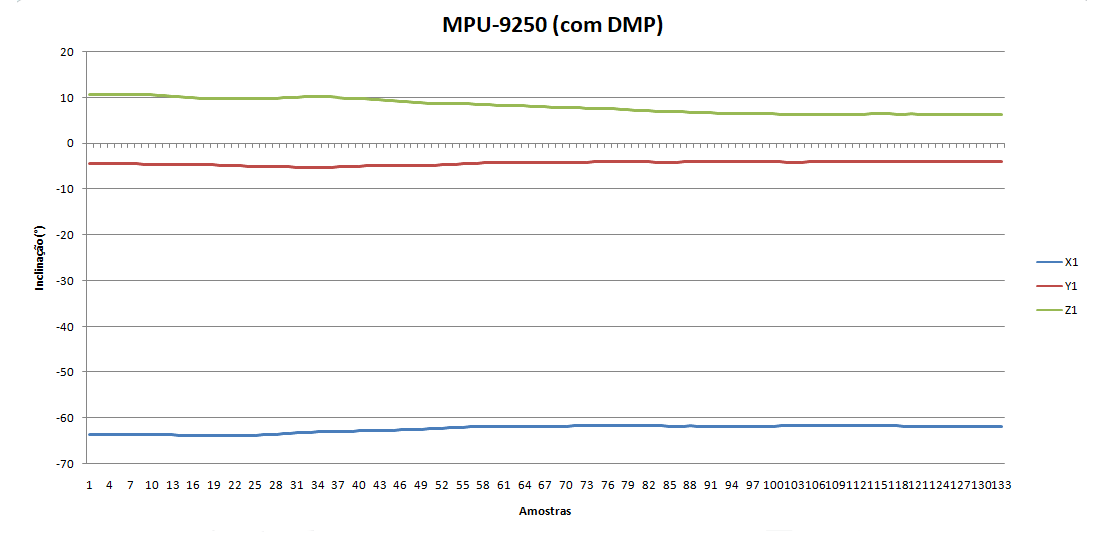
\includegraphics[height=.4\textheight]{figs/9250dmp_plano.png}
      \tiny{\textbf{\\Fonte: Autor}}
    \end{column}
  \end{columns}
}

\frame{
  \frametitle{Análise Estatística}
  \note[item]{dados obtidos mantendo cada posição por 10 segundos, repetindo 3 vezes}
  \note[item]{Desvio Padrão e Amplitude mais baixos demonstra os benefícios da aplicação do filtro}
  \note[item]{DMA mais baixo indica maior precisão dos movimentos}
  \begin{columns}
    \begin{column}{\paperwidth}
      \centering
      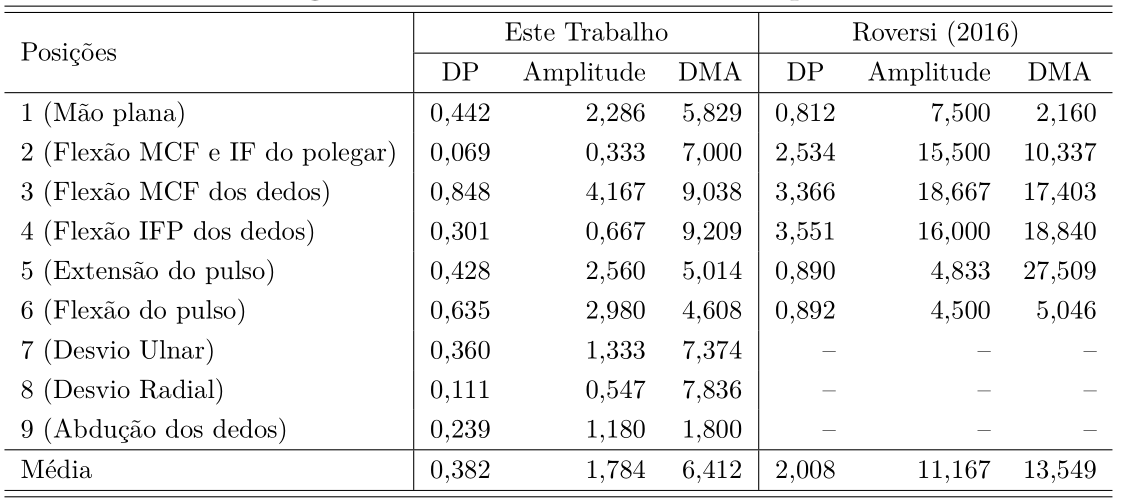
\includegraphics[height=.6\textheight]{figs/tabela.png}
      \tiny{\textbf{\\Fonte: Autor}}
    \end{column}
  \end{columns}
}

\frame{
  \frametitle{Posições}
  \begin{columns}
    \begin{column}{\paperwidth}
      \centering
      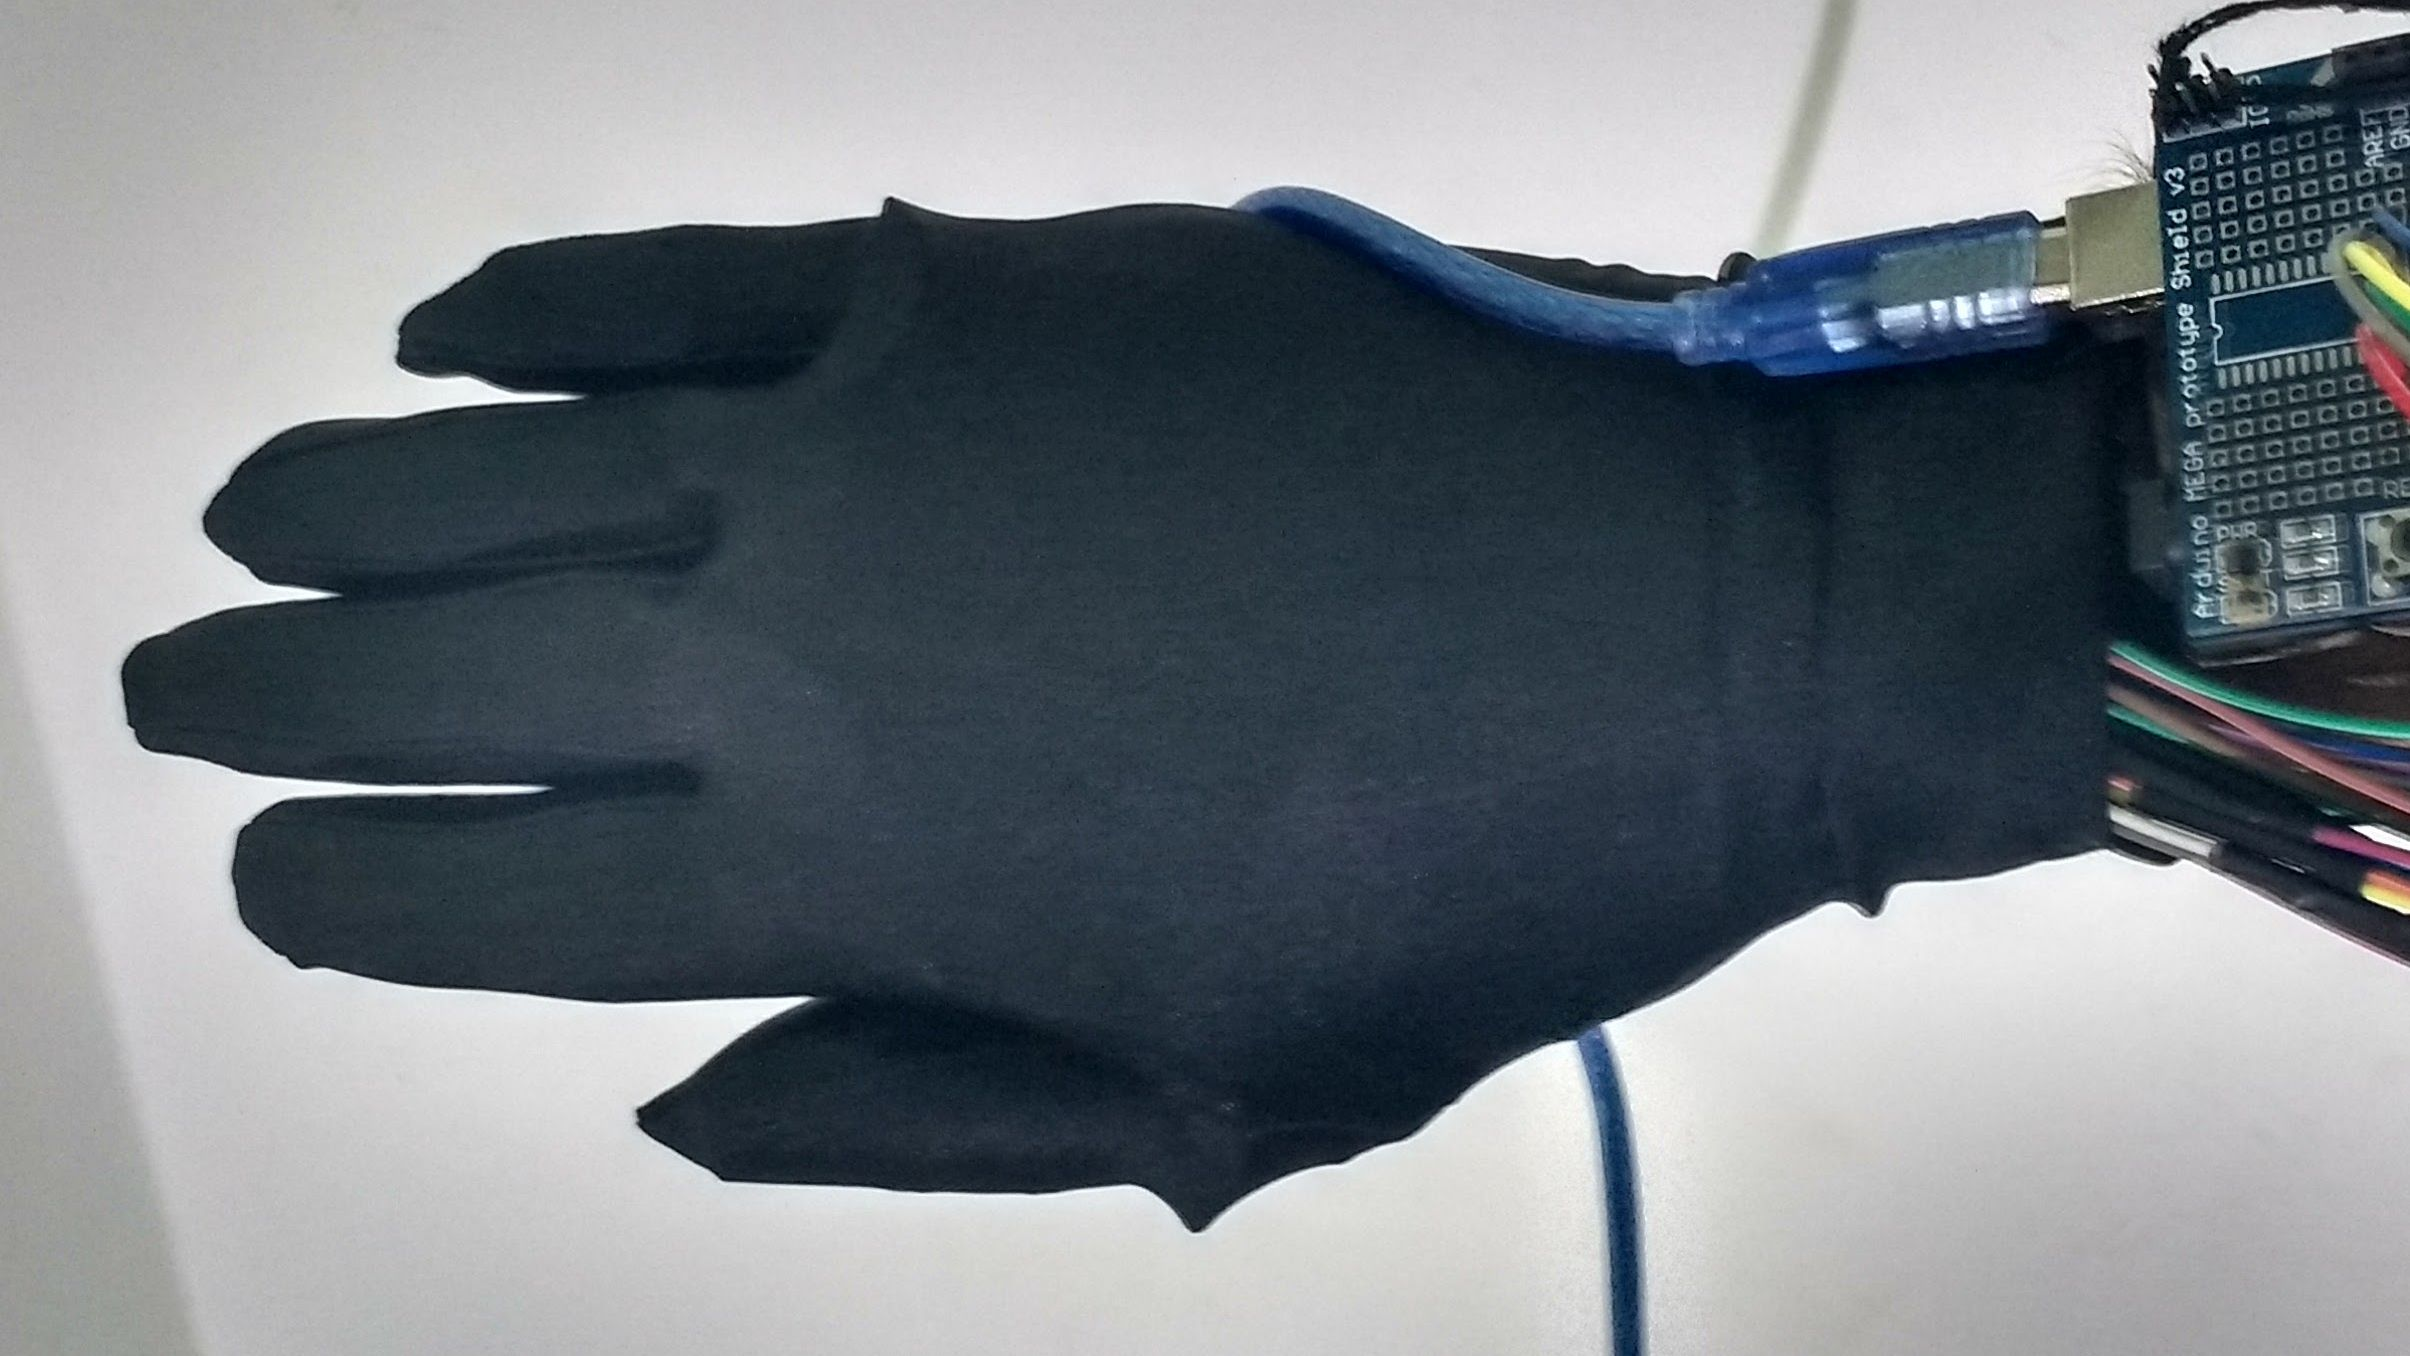
\includegraphics[height=.3\textheight]{figs/p1_real.jpg}
      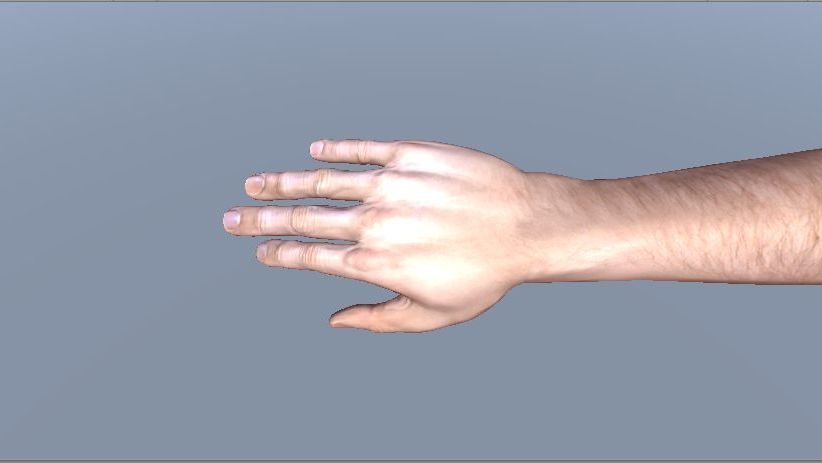
\includegraphics[height=.3\textheight]{figs/p1.jpg}\\
      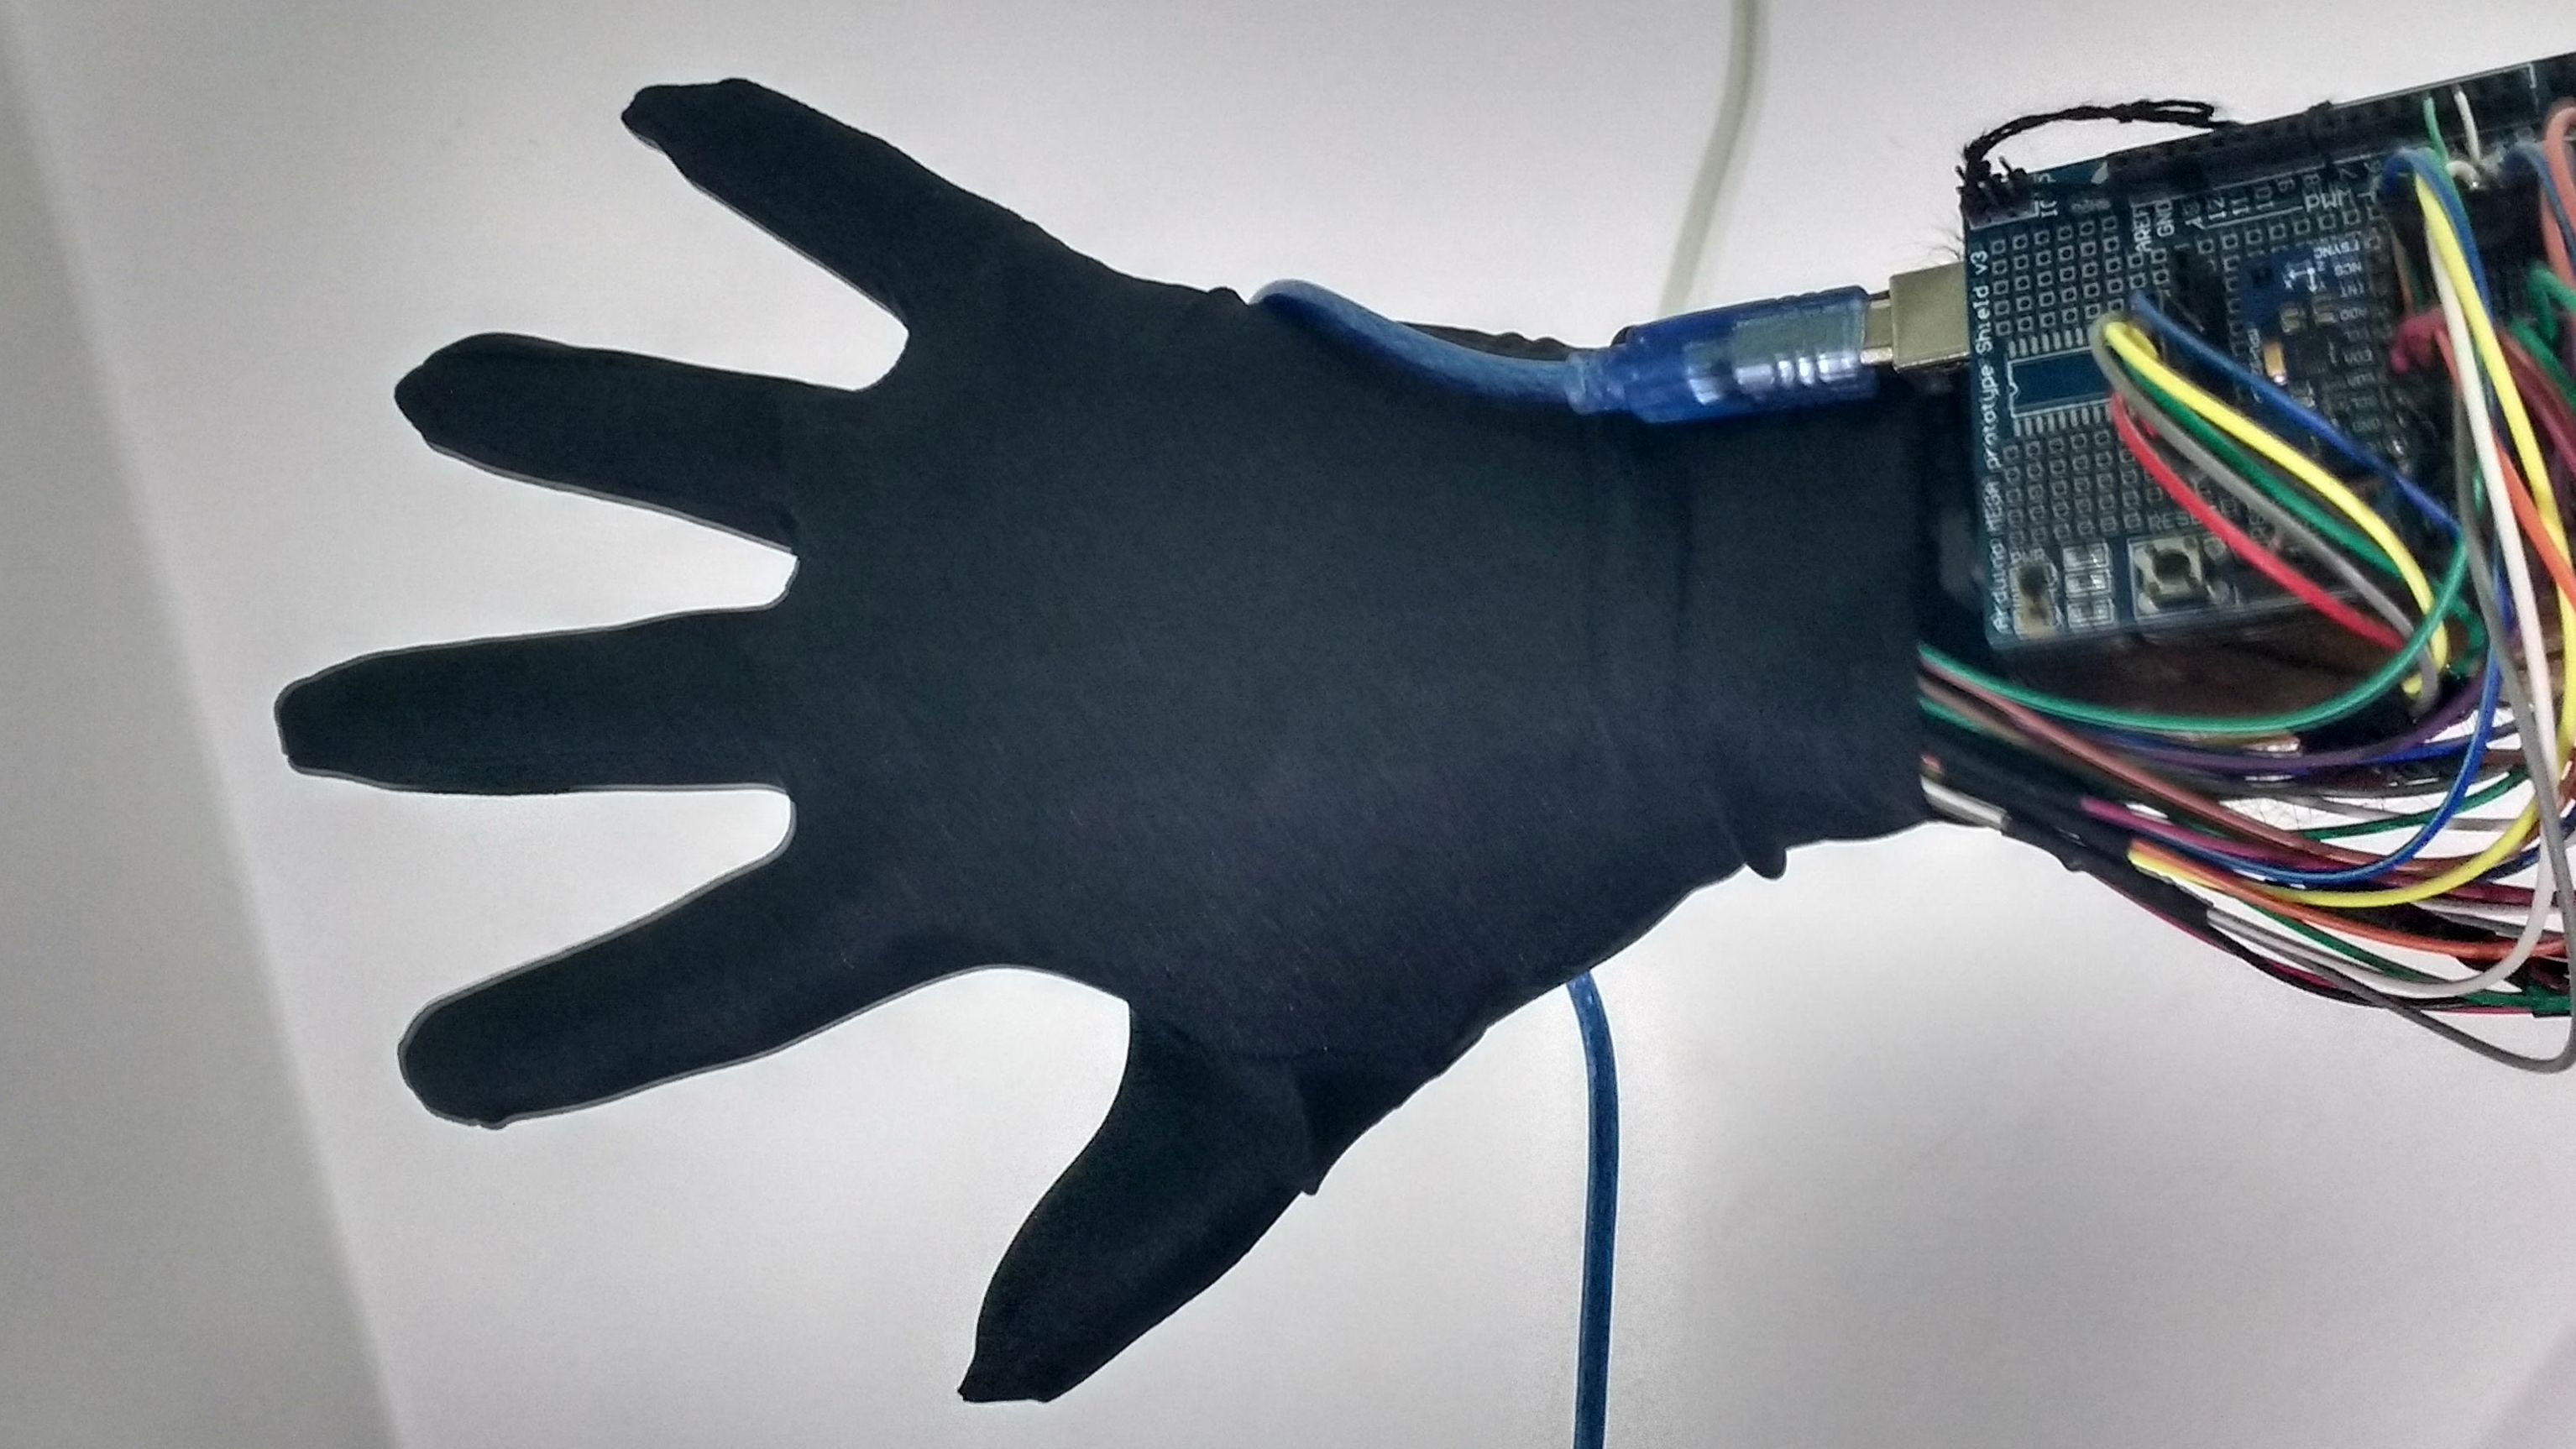
\includegraphics[height=.3\textheight]{figs/p9_real.jpg}
      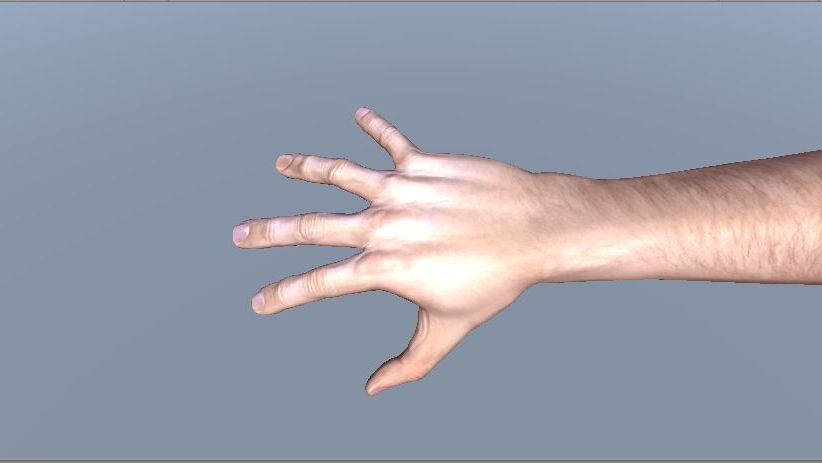
\includegraphics[height=.3\textheight]{figs/p9.jpg}
      \tiny{\textbf{\\Fonte: Autor}}
    \end{column}
  \end{columns}
}

\frame{
  \frametitle{Posições}
  \begin{columns}
    \begin{column}{\paperwidth}
      \centering
      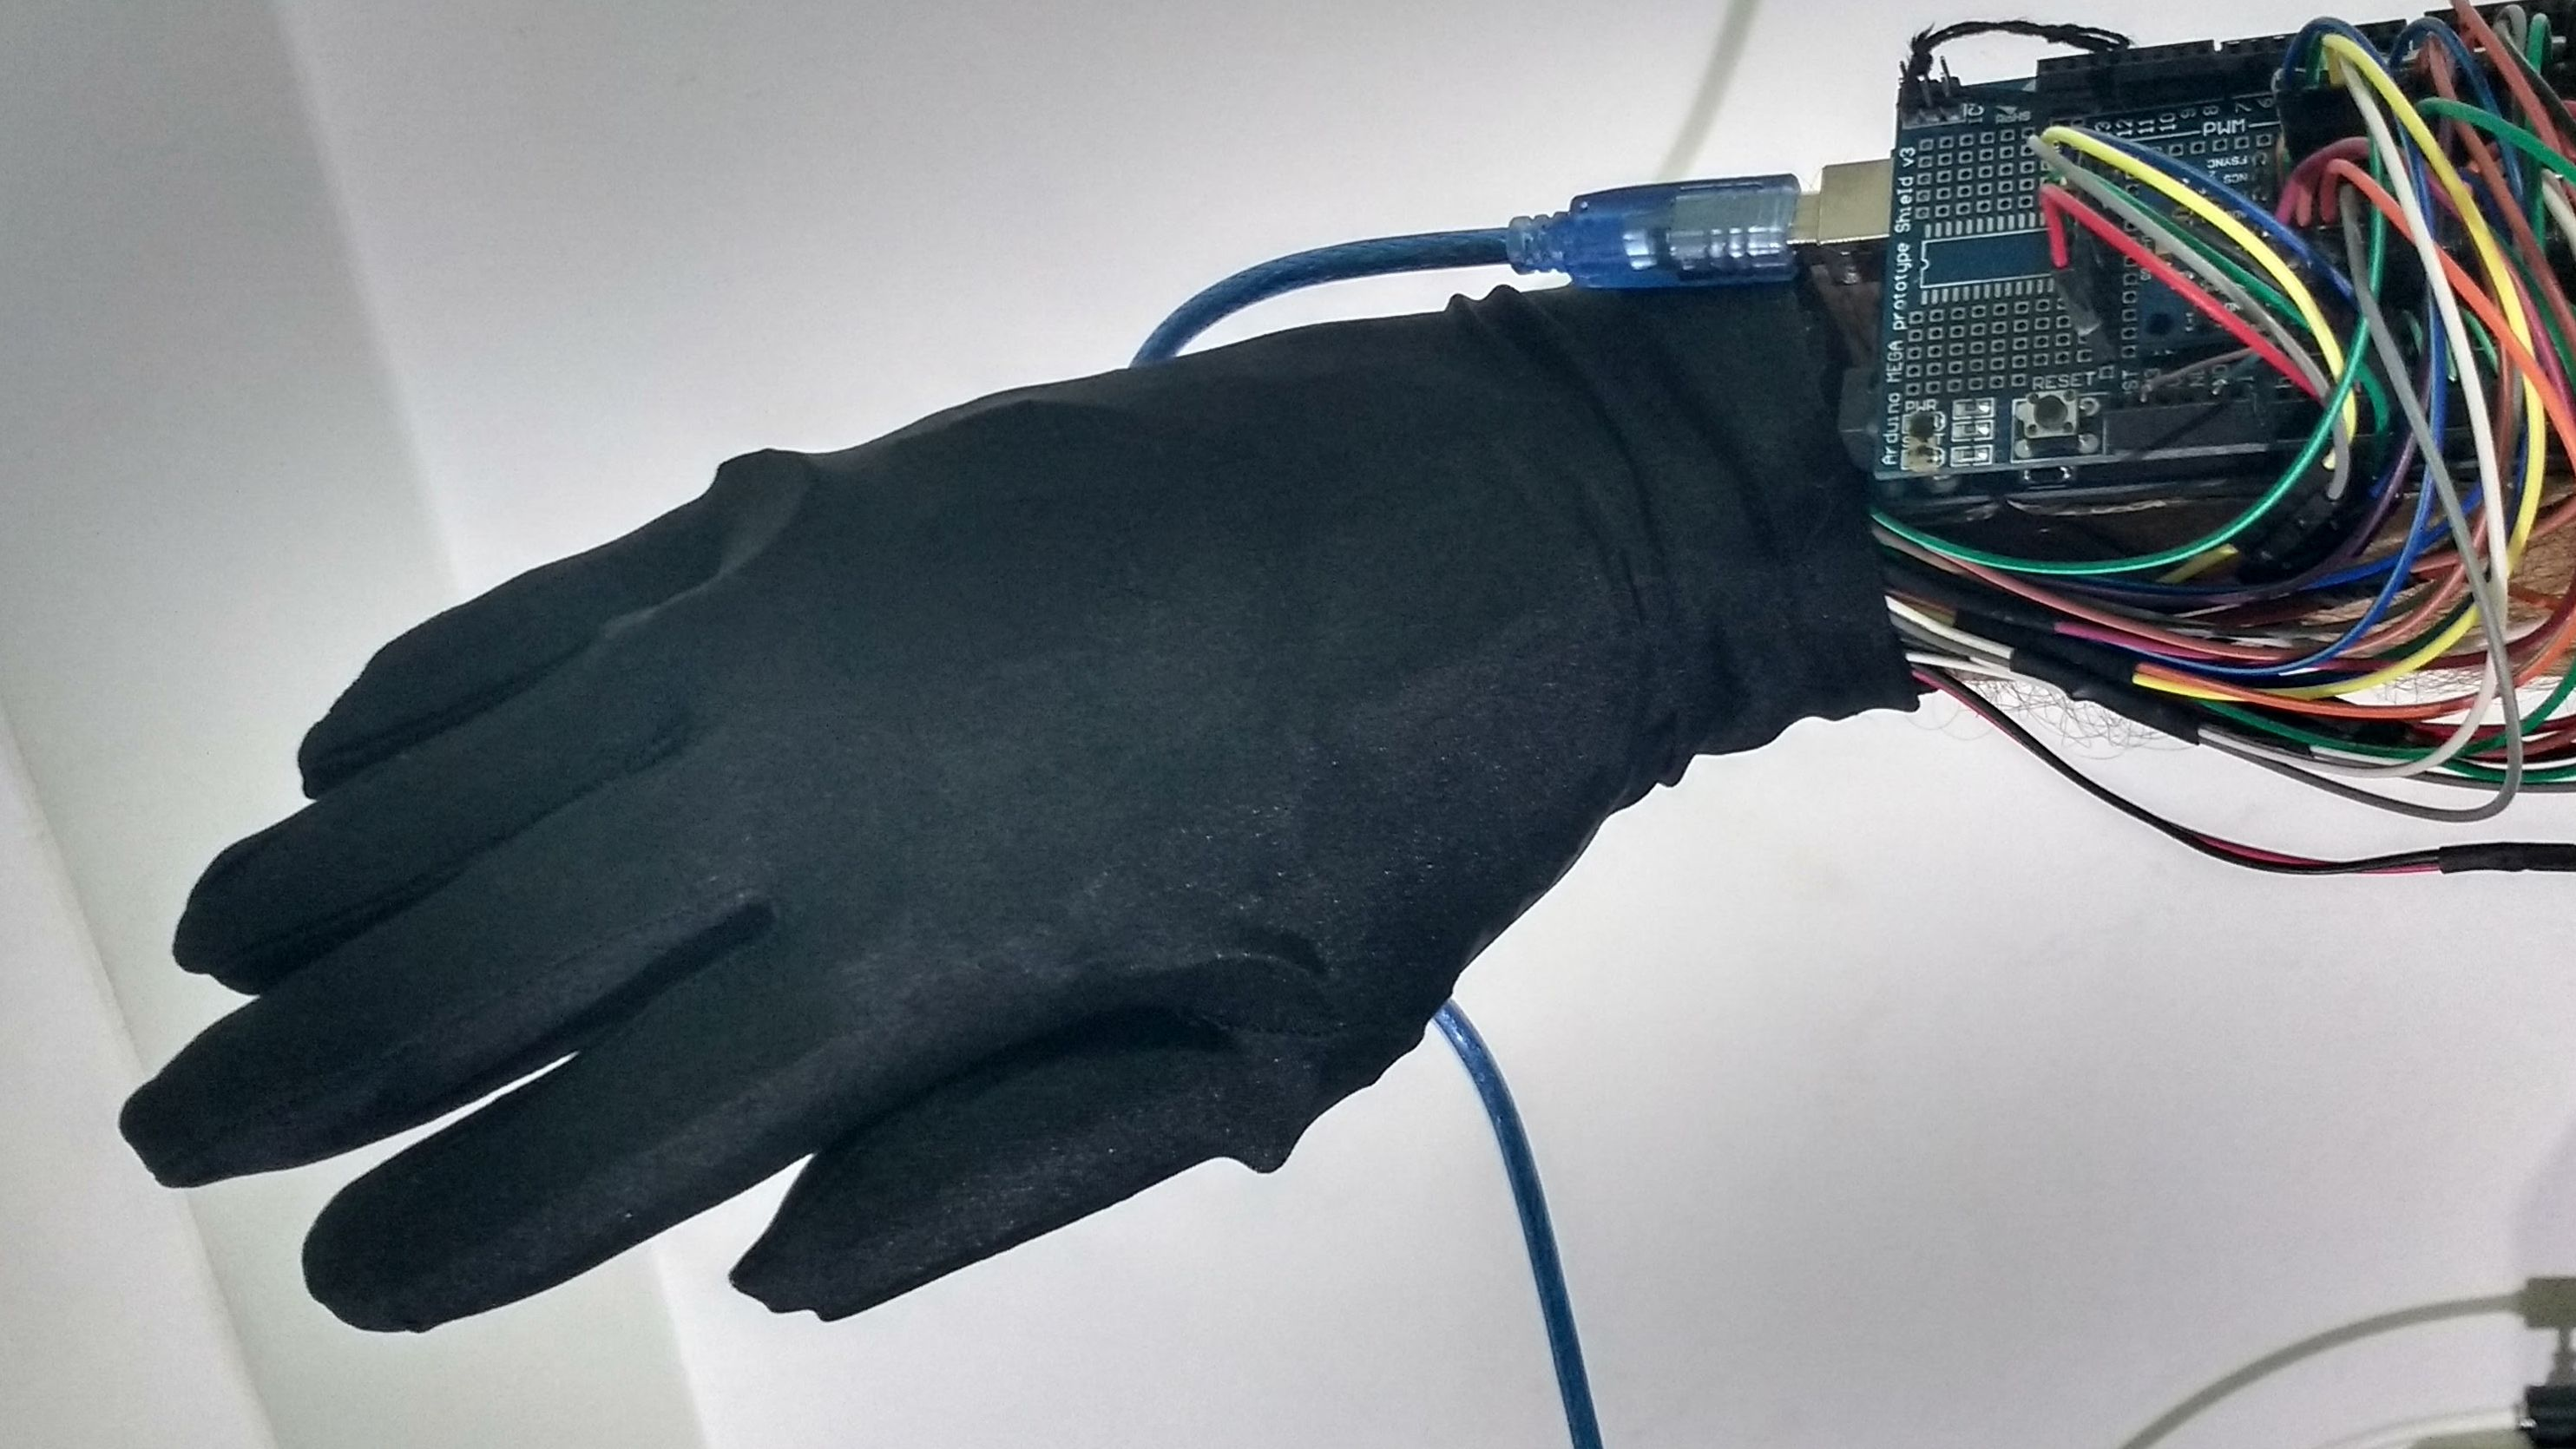
\includegraphics[height=.3\textheight]{figs/p7_real.jpg}
      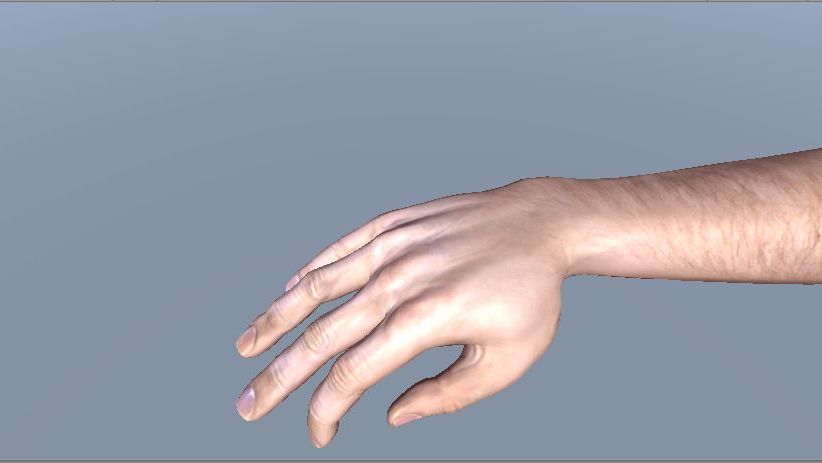
\includegraphics[height=.3\textheight]{figs/p7.jpg}\\
      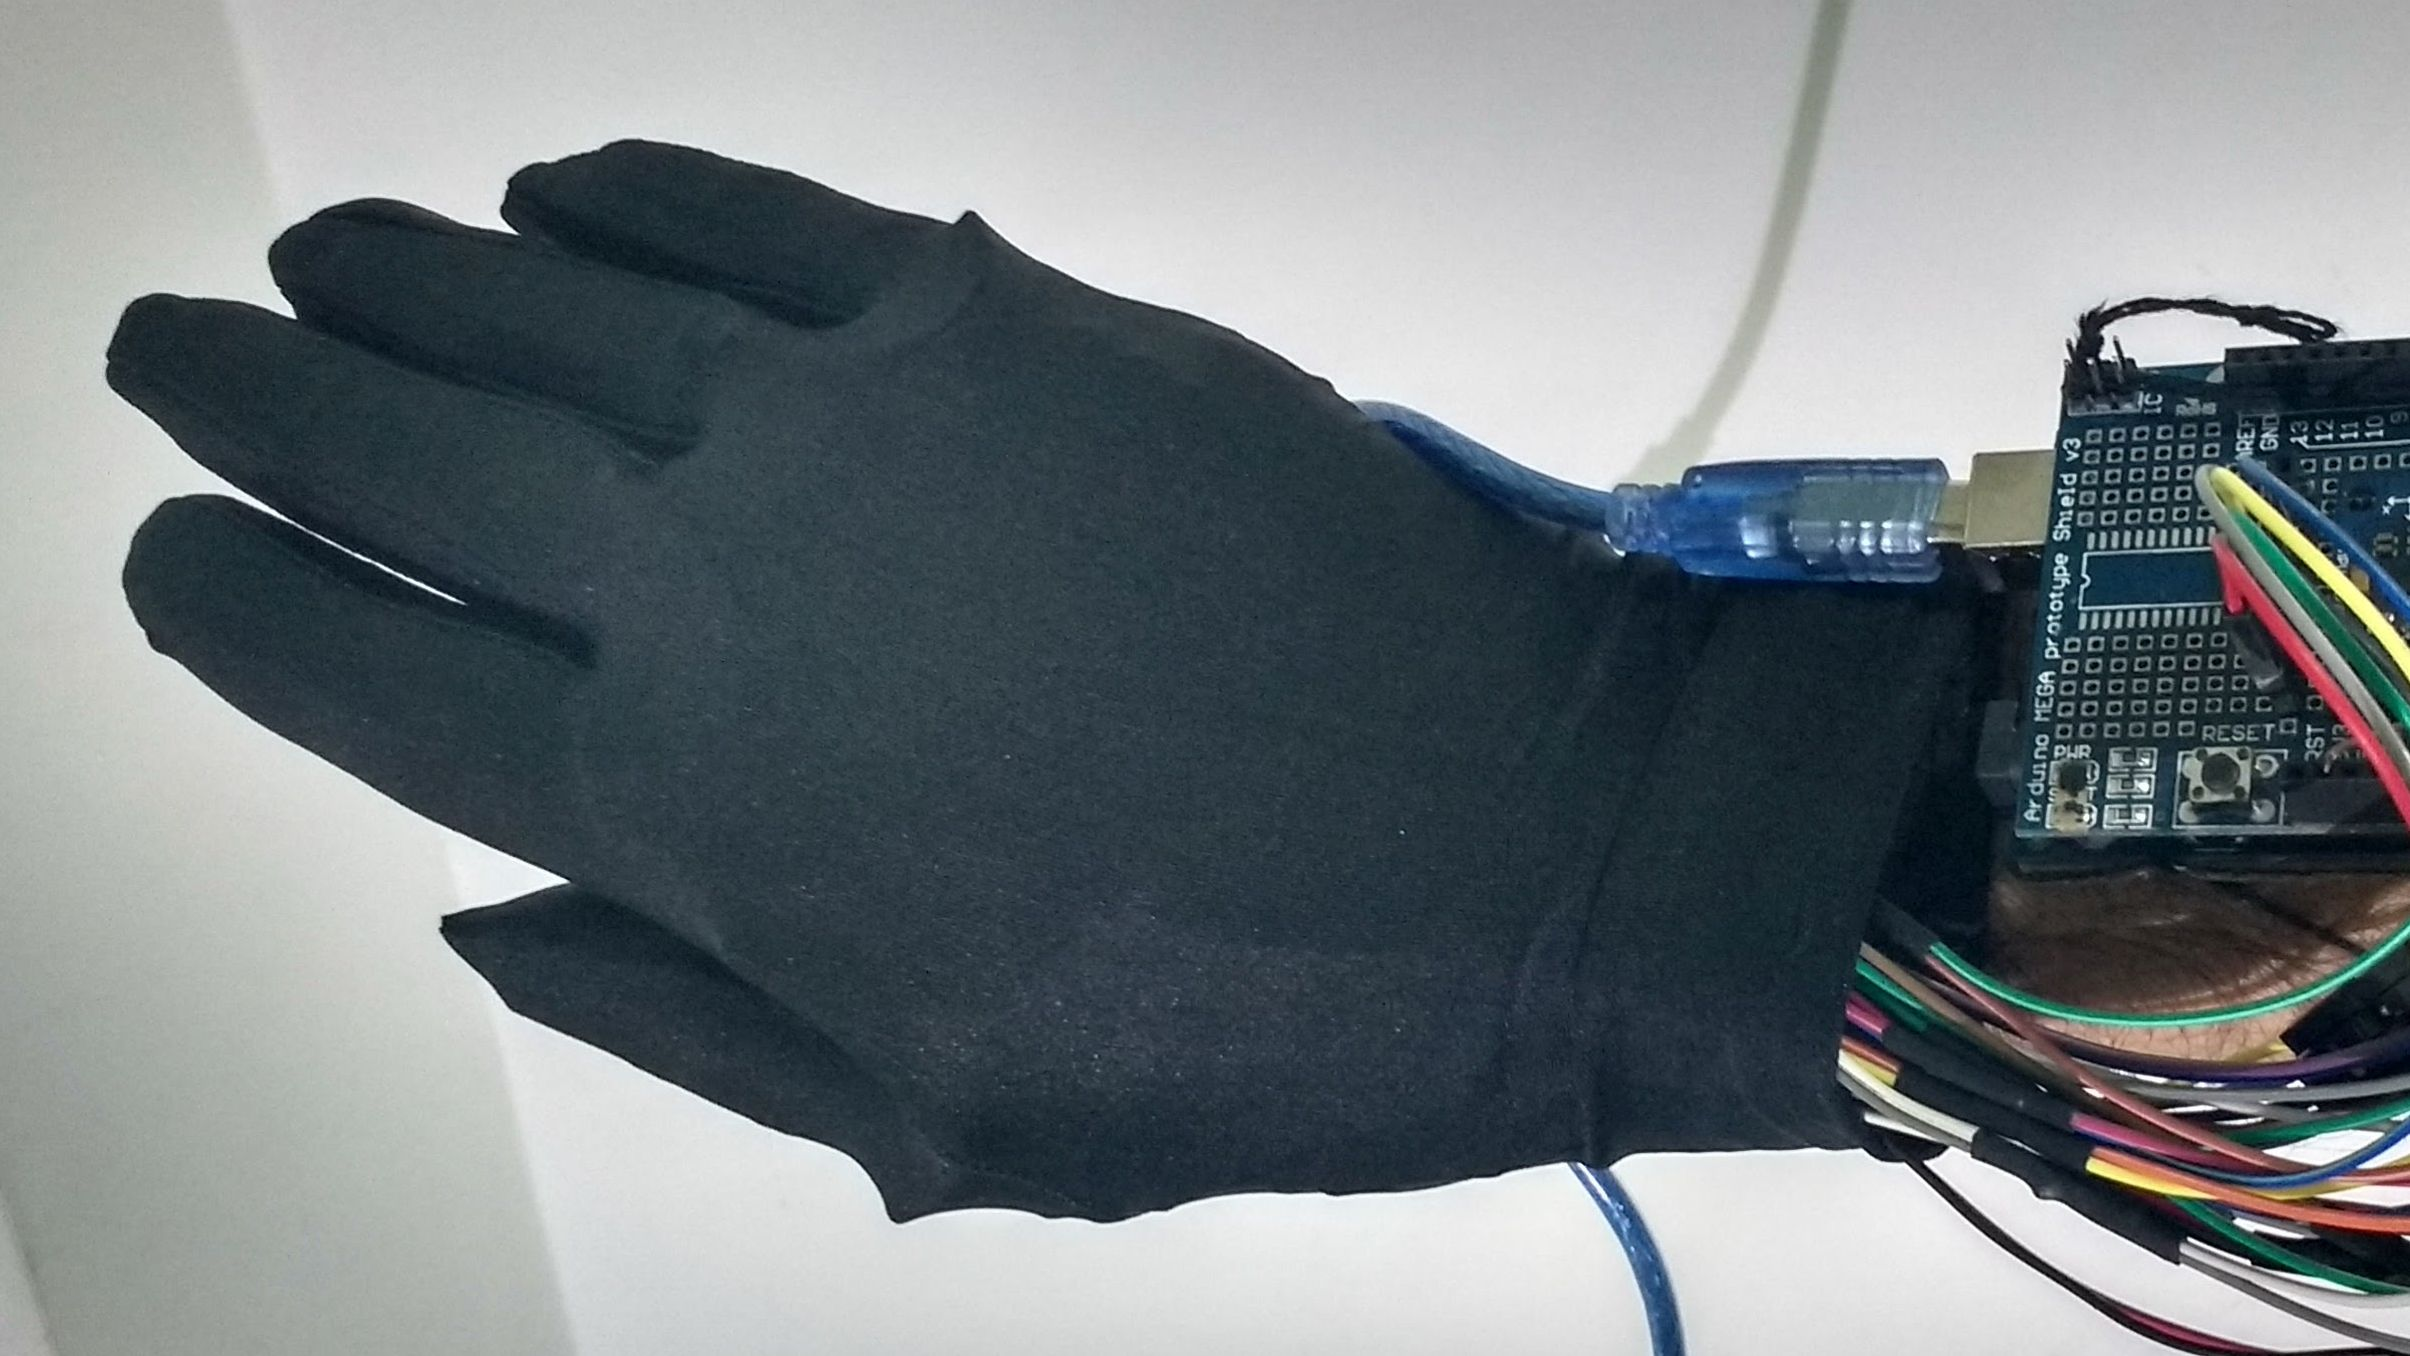
\includegraphics[height=.3\textheight]{figs/p8_real.jpg}
      \includegraphics[height=.3\textheight]{figs/p8.jpg}
      \tiny{\textbf{\\Fonte: Autor}}
    \end{column}
  \end{columns}
}

\frame{
  \frametitle{Demonstração}
  \centering
  \movie[externalviewer]{\includegraphics[width=\textwidth]{figs/thumbnail}}{vid/Video_TD.mpg}
}

\section{Conclusões e Trabalhos Futuros}
\frame{
  \note[item]{Problemas encontrados incluem cabo USB atrapalhando movimentos conexões falhando, etc...}
   \frametitle{Conclusões}
    \begin{itemize}
      \item Colocação e remoção da luva foi difícil devido ao material utilizado;
      \item Movimentos pequenos dos dedos não foram captados;
      \item Movimentos de adução e abdução do dedo médio não foram captados;
      \item Foram captados os movimentos de desvio radial e ulnar do pulso;
      \item A redução de ruídos dos sensores foi satisfatória.
    \end{itemize}
}

\frame{
   \frametitle{Trabalhos Futuros}
   \begin{columns}
     \begin{column}{.7\textwidth}
       \begin{itemize}
          \item Luva de material diferente;
          \item Melhor fixação do \textit{Arduino} no braço;
          \item Sensores de flexibilidade com maior resolução.
          \item Detecção de mais movimentos;
        \end{itemize}
     \end{column}
     \begin{column}{.3\textwidth}
        \centering
        \includegraphics[width=\textwidth]{figs/thumb-workings.jpg}
        \tiny{\textbf{\\Fonte: \citeonline{movimentos}}}
     \end{column}
   \end{columns}
    
}


\section{Referências}
\begin{frame}[allowframebreaks]{Referências}
    \frametitle{Referências}
  \begin{tiny}
    \bibliography{apresentacao}
  \end{tiny}
\end{frame}

\begin{frame}[t]
\centering
\pgfuseimage{inic}\\
\titlepage
\end{frame}
\end{document}